%
\section{\color{red}Introduction\label{ptInt}}

%
The perspective of Beverton-Holt \cite{beverton_dynamics_1957} has been 
foundational to the structure of modern fisheries models \cite{holden_beverton_1995}. 
Evolving from the work of Von Bertalanffy \cite{von_bertalanffy_quantitative_1938}, 
alongside the Ricker \cite{ricker_stock_1954} and Schaefer \cite{schaefer_study_1957}   
models, the perspective of Beverton-Holt shaped the following decades of fisheries 
research. To this day, stock assessments view the BH model of recruitment as a 
default \cite{methot_stock_2013, barnes_stock_2023}. %, black}. 

%{\color{red} add black rockfish assessment assessment}

% and ricker \cite{ricker} models 
% and varied history 
%\begin{itemize}
%\item gotelli, 2001 ecology book (density dependence)
%\item appaears in stock assessments \cite{ss3}, \cite{black} \cite{other assessments of the last cycle?}
%\item control theroy \cite{}
%\item motivate pervasive BH \cite{holden}
%%Holden, Mike. “Beverton and Holt Revisited.” Fisheries Research 24, no. 1 (July 1, 1995): 3–8. https://doi.org/10.1016
%\item maunder BH density dependence paper
%\end{itemize}

%model approaches the recruitment relatiohship with a quadratic nonlinear differential equation. 
%However in the BH model they essentially model $\frac{dP}{dt}$ with a 
%quadriatic logistic model
%
%%and an independent handling of recruitment. 
%
%%modeling %for assumes a quadriatic logistic differential equation 
%
Similarly to the Schaefer model, the Beverton-Holt (BH) model 
\cite{beverton_dynamics_1957} is founded on a notion of density 
dependence \cite{gotelli_primer_1995} (albeit to a lesser extent). 
%Like the Schaefer model, the BH model begins the derivation of their 
Unlike the Schaefer model, the BH approach to modeling productivity factors the 
density dependance related to recruitment separately from terms relating to 
natural mortality, behooving a more explicit model of natural mortality \cite{beverton_review_1959}.
%This behooves an additional and more explicit model of 
%natural mortality \cite{beverton_review_1959} while recruitment is modeled separatly. 
Similarly to the Schaefer model, there derivation of the recruitment 
relationship assumes that density dependence appears as a quadriatic logistic 
differential equation. However the BH model formulates this as a model of the 
change in recruitment over time, rather than as a direct model of net productivty 
as seen in the Schaefer model. They then solve this equation in discrete time 
and reparameterize to argue for the generality of the resulting recruitment 
relationship that we use today. 

%
For purposes of this study their recruitment relationship is 
reparameterized as, % consider the % By solving this differential equation they derive 
%
\begin{equation}
P(B) = \frac{\alpha B}{1+\beta B}.
\end{equation}
%
The parameter $\alpha$ here has a similar interpretation as the $r$ parameter, 
from the Scheafer model, in that it represents the slope at the origin of the 
production function. The $\beta$ parameter here is also related to $K$, 
from the Scheafer model, however the BH model is not parameterized 
directly in terms of carrying capacity but rather $K\propto\frac{1}{\beta}$. 
The primary role of $\beta$ in this parameterization is to scale the 
population, and $\beta$ is largly responsible for controling carrying capacity 
in practice. 

\begin{figure}[h!]
\begin{minipage}[h!]{0.49\textwidth}
        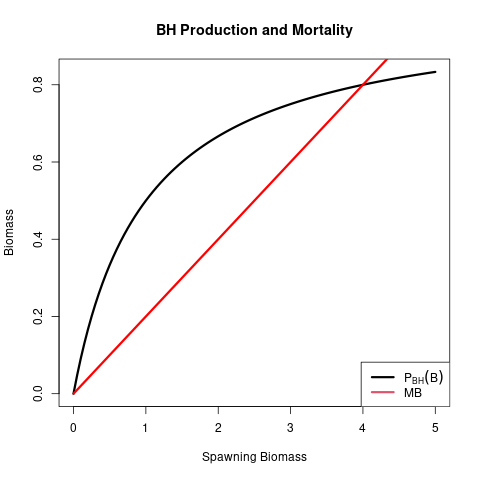
\includegraphics[width=\textwidth]{../gpBias/pBHandM.png}
\end{minipage}
\begin{minipage}[h!]{0.49\textwidth}
	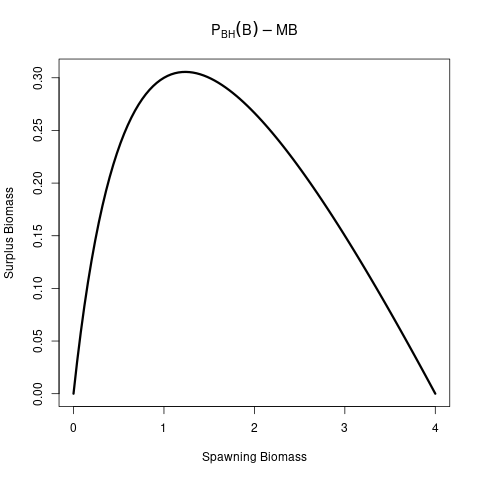
\includegraphics[width=\textwidth]{../gpBias/yeildBH.png}
\end{minipage}
\caption{\label{srrBH}
	($left$) BH production function plotted along side a linear model of natural mortality.
	($right$) Surplus production implied by the combined BH model of production and linear natural mortality.
	%\color{red} Thou shlt write me a caption
       % \\The logistic production function in black plotted next to depictions of the key biological parameters and ref
       % The slope at the origin (and thus $r$) is shown in blue, catch resulting in MSY in red, biomass at MSY in green
       % MSY is seen at the peak of the parabola, and is attained with a fishing rate of $\frac{r}{2}$ and biomass equil
}
%\end{wrapfigure}
\end{figure}

%
As seen in Figure (\ref{srrBH}, $left$) the BH model is an asymptoing curve, 
such that as $\lim_{B\to\infty}P_{BH}(B)=\frac{\alpha}{\beta}$. This makes the 
inclusion of an explicate handling of natural mortality, $M$, pertinent for 
the modeling of surplus production. In this case, $MB$ represents linear natural 
mortality, but it also constitues a replacement line where biological production 
must exceed this rate of mortality to persist. Figure (\ref{srrBH}, $right$) 
demonstrates how when the typical linear handling of natural mortality is 
taken together with the BH model a left leaning surplus production curve is 
produces that is reminiscent of PT curves for $\gamma_{PT}<2$ as can be seen in 
Figure (\ref{SrrPT}).
  
%{\color{red} talk about including $M$, plot BH and M and then yeild with RPs}
%{\color{red} Something about the limitations of RPs \cite{mangel_perspective_2013, brooks_analytical_2010} }

%
Under the PT model recall when $\gamma_{PT}\le2$ the RPs lie in the lower 
$\frac{B^*}{B_0}\le0.5$ region of RP space. Under the BH model this is also the 
case, although due to two-parameter form of the BH model, the set of BH RPs is a 
curve passing through $\frac{B^*}{B_0}\le0.5$. Myers et. al. \cite{myers_maximum_1999}, 
Brooks et. al. \cite{brooks_analytical_2010}, and Mangel et. al. \cite{mangel_perspective_2013} 
show how this limitation arrises analytically via steepness. Mangel et. al. \cite{mangel_perspective_2013}, 
further demonstrates the generality of this phenomena, and shows how these 
functional limitations limit fisheries managment based on $MSY$-based RPs. 
%numerous softer correlation examples Williams (2002), Punt et al. (2008), and Brooks et al. (2010).
%Brooks and Powers (2007), Forrest et al. (2010) 

%
Deriso \cite{deriso_harvesting_1980} and Schnute \cite{schnute_general_1985} 
developed slightly different (but conceptually equilavent) three-parameter 
generalizations of the BH model
\footnote{
The later form in \cite{schnute_general_1985} is prefered here due its 
interpretability and the improved regularity of closed form RPs it produces.
}.
This model generalizes the BH model by controlling the nature of density 
dependence by allowing production to increase or decrease beyond that of the 
BH model for large spawning biomass. 
%
The Schnute model not only generalizes the BH model, but in doing so it 
frees the RP limitations presented above. The three-parameter Schnute model has 
the two-parameter BH, Ricker, and Schaefer models, as special cases. 
Each of the two-parameter models limits RPs similarly to the BH model, but in 
particular each of them models a different set of RPs. 
As the Schnute model transitions between these models it takes intermediate 
forms which can model all of the interviening RPs, thus representing all of 
the most biologically relavant hypotheses commonly discussed in fisheries 
management.  

%
In this chapter the Schnute model is used to generate index data simulated 
broadly in RP-space but fit with an intentionally misspecified BH model. This
%parameterizes %simulated 
parameterizes a broad set of misspecified situations for the BH model
where the simulated data have well understood dynamics in the fisheries
community. A GP metamodel of the simulation demonstrates how misspecification 
of the BH model forms biases in RP estimation. First, as many as possible of 
the neccessary %some of the neccessary 
RP expressions are derived analytically under the Schnute model. The remaining 
RPs do not have analytical expressions. Therefore, a numerically stable method 
is then developed that allows an adaptive simulation design to be computed 
without the remaining closed-form RP expressions. The GP metamodel (as 
developed in Section (\ref{gpmm})) is then used to demonstrate the nature of RP 
biases under the BH model. 
%is controlled by the information content in the data.


%{\color{blue}
%
%%
%The Deriso production function presents a convenient three parameter form
%that is capable of representing many of the most common two parameter production
%functions as special cases \cite{deriso_harvesting_1980}. The BH and
%Logistic production functions arise when $\gamma$ is fixed to -1 or 1
%respectively, and the Ricker model is a \mbox{limiting case as
%$\gamma\rightarrow0$ \cite{schnute_general_1985}.}
%
%%
%Using the Deriso model as a data generating model across a wide range
%of RP-space, similarly as described in Section (\ref{sim}), %, and fitting those data under a BH model, 
%presents an ideal setting for extending the above study of RP biases across a
%broad range of productivity assumptions. Under the Deriso model inverting the
%relationship between RPs and model parameters is not fully analytically possible
%\cite{schnute_analytical_1998}. Numerical inversion of the nonlinear system
%seen in Eq (\ref{system}) is required for determining parameter values for data
%generation. Notice for a given $\gamma$ value, $\alpha$ and $\beta$ can be
%solved analytically.
%
%%While the Deriso model generalizes many common models, inference under 
%Inference under the BH model is of particular interest due to its overwhelming
%popularity in stock assessment. Similar to the limited RP-space of the
%Schaefer model the two parameter BH model also has a limited RP-space as shown
%in Figure (\ref{bhRP}).  While the BH constrained RP space is more complicated
%than the Schaefer model, analogy to the results obtained under the
%PT-Schaefer simulation setting, and the flexible GP metamodel, should expedite
%the analysis of BH inference.
%
%}

%{\color{gray}
%%%
%%The PT model is a three parameter generalization of the Schaefer model that uses
%%its extra parameter to explicitely control the location of $\frac{B^*}{\bar B(0)}$.
%%In doing so, the PT model can model the entire space of RPs and does so in a way that
%%retains much of the analytical appeal of the Schaefer model. While there are some oddities
%%of the functional form \cite{punt_extending_2019, fletcher_restructuring_1978}, the model
%%has been very useful in generalizing the analysis of RPs \cite{winker_jabba_2018}.
%
%%
%In this chapter the PT model is used to generate index data simulated broadly
%in RP-space but fit with an intentionally misspecified Schaefer model. This
%%parameterizes 
%%simulated 
%parameterizes a broad set of misspecified situations for the Schaefer model
%where the simulated data have well understood dynamics in the fisheries
%community. A GP metamodel of the simulation is developed to demonstrate how
%misspecification of the Schaefer model forms biases in RP estimation. First,
%analytical expressions for RPs are derived under the PT model for use in
%deriving a fully analytical simulation design. Next, a GP metamodel is
%developed and a catch is parameterized in terms of contrast to demonstrate
%how the nature of bias is controlled by the information content in the data.
%}

%{\color{red}
%\begin{itemize}
%%\item history of BH
%%\item motivate pervasive BH \cite{holden}
%%Holden, Mike. “Beverton and Holt Revisited.” Fisheries Research 24, no. 1 (July 1, 1995): 3–8. https://doi.org/10.1016/0165-7836(95)00377-M.
%%\item maunder BH density dependence paper (2022)
%%\item Hamel, maunder Natural mortality (2023)
%%\item Pauly: M and individual growth 
%\item gotelli, 2001 ecology book (density dependence)
%%
%\item what is Schnute all about
%\item take a paragraph from advancment
%\item Under the Deriso model inverting the relationship between RPs and model parameters is not fully analytically possible \cite{schnute_analytical_1998}
%\end{itemize}
%}

%
\section{Methods \label{meth}}


%
\subsection{Model\label{sModel}}

%
The Schnute production function is a three-parameter generalization of many of
the most common two-parameter production functions \cite{deriso_harvesting_1980, schnute_general_1985}. %\shortcit{deriso_harvesting_1980}. 
It can be written in the following form, with parameters $\alpha$, $\beta$, and $\gamma$,
%
\begin{align}
P_s(B; [\alpha, \beta, \gamma]) = \alpha B (1-\beta\gamma B)^{\frac{1}{\gamma}}.
\end{align}

%
\begin{wrapfigure}{r}{0.5\textwidth}
%\begin{figure}[h!]
%\begin{minipage}[h!]{0.64\textwidth}
\vspace{-0.6cm}
%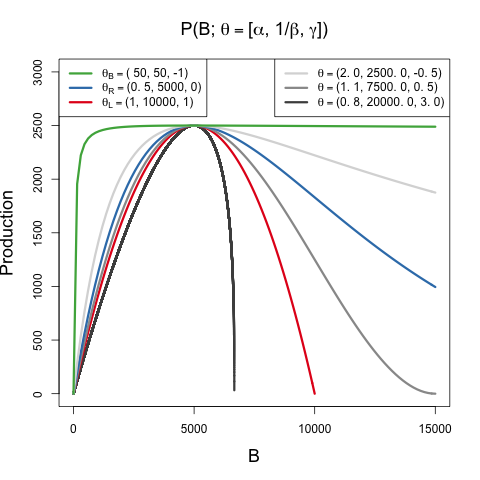
\includegraphics[width=0.5\textwidth]{plots/derisoSrr.png}
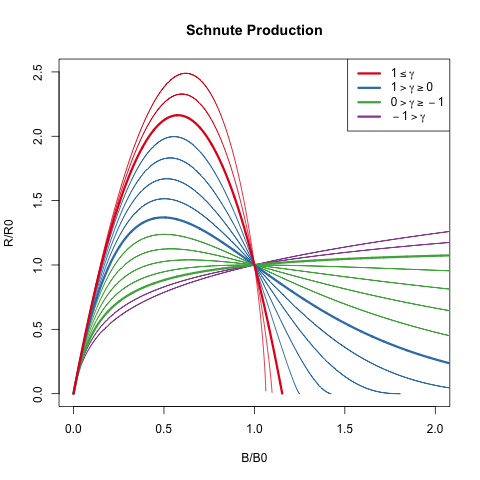
\includegraphics[width=0.49\textwidth]{../gpBias/g3.png}
\vspace{-1cm}
%\end{minipage}
%\begin{minipage}[h!]{0.3\textwidth}
\caption{
%\onehalfspacing
The Schnute production function plotted across a variety of parameter
values. Regimes of similarly behaving curves are grouped by color.
% BH-like, Ricker-like, and Logistic production are shown in
%green, blue, and red respectively.
}
\label{sRegimes}
%\end{minipage}
\end{wrapfigure}
%\end{figure}

%
The BH and Logistic production functions arise when $\gamma$ is fixed to -1 or
1 respectively. The Ricker model is a limiting case as $\gamma\rightarrow0$. %\shortcite{schnute_general_1985}.
For $\gamma<-1$ a family of strictly increasing Cushing-like \cite{cushing_dependence_1971} 
curves arise, culminating in linear production as $\gamma\to-\infty$. These 
special cases form natural regimes of similarly behaving production functions 
as seen in Figure (\ref{sRegimes}).

%
The behavior of RP inference under the BH model is of particular interest due
to the overwhelming popularity of the BH assumption in fisheries models.
%% 
%Inference of BH productivity parameters under a wide variety of data is of particular 
%interest due to the overwhelming popularity of the BH assumption in fisheries 
%models. 
Since Schnute production models can represent a quantifiably wide variety
of possible productivity behaviors, they present an ideal simulation
environment for inquiry of the reliability of inference under the BH
assumption.


%
Under Schnute production, biomass dynamics evolve according to the following ODE,
%
\begin{align}
\frac{dB}{dt} = P_s(B;\theta) - (M+F)B. \label{schnuteSimple}
\end{align}
%
This equation largely takes the same form as previously described, except
that $P_s$ is the Schnute production function and natural mortality, $M$, is modeled
explicitly here. % as opposed to  inclusion of natural mortality, $M$. 
Natural mortality models the instantaneous rate of mortality from all causes
outside of fishing. While Eq. (\ref{schnuteSimple}) models $M$ explicitly,
natural mortality is implicit to the structure of the previously decribed
Schaefer, Fox, and PT production models. Explicitly modeling natural mortality 
in this way allows $P_s$ to model the production function in such a way so as to allow 
production to increase for large spawning biomass (or asymptote, e.g. BH production), 
and still retain well defined RPs so long as $\alpha>M$. % well defined. %This is not only a typical assumption
%biomasses (e.g. BH production). In turn, the Schunte model requires the addition
%of the term $-MB$ to form an interpretable yeild curve and make RPs well defined
%over the relevant domain of $\gamma$.
This handling of $M$ is typical for age structured models under BH or Ricker 
recruitment (or even BH/Ricker production models), but it is uncommonly used with the 
Schaefer model ($\gamma=1$) as is possible in this setting. Appendix (\ref{mApp}) 
shows that while explicite $M$ may not be typical under the Schaefer model, the 
assumption of linear natural mortality, $-MB$, produces a mathematically valid 
Scheafer model with an admissible interpretation.  
%some values of $\gamma$ may lead to the logistic {\color{red} [logistic 
%model]-MB=[another logistic model] with slightly different 
%parameterization such that M is explicite. parabola-parabola is another parabola.}

%is not only a typical assumption of fisheries models, but is also key to the making 
%RPs well defined over the relevant domain of $\gamma$.

%% matches the assumptions of typical fisheries models and 
%%
%In the Schaefer and PT models
%$M$ is modeled explicitly here  and $F$ are instantaneous rates of natural and fishing 
%mortality respectively. Unlike the PT model described above 

%with Schnute production simulates a
%wide variety of possible population productivity behaviors and provides an 

%
The derivation of RPs under Eq. (\ref{schnuteSimple}) follows a similar logic
as under the PT model. An expression for equilibrium biomass is attained by
setting $\frac{dB}{dt}=0$ and rearranging the resulting expression to solve
for $B$
%
\begin{align}
\bar{B}(F) &= \frac{1}{\gamma \beta}\left(1-\left(\frac{M+F}{\alpha}\right)^\gamma\right).
\label{BsEq}
\end{align}

%
The above expression quickly yields $B_0$, $B^*$ by evaluation at $F=0$ and $F^*$ respectively,
%derive \bar B(F)
\begin{align}
B_0 &= \frac{1}{\gamma \beta}\left(1-\left(\frac{M}{\alpha}\right)^\gamma\right) \label{B0S}\\
\frac{B^*}{B_0} &= \frac{1-\left(\frac{M+F^*}{\alpha}\right)^\gamma}{ 1-\left(\frac{M}{\alpha}\right)^\gamma }. \label{BratS}
\end{align}


%
Attaining an expression for $F^*$ requires maximization of equilibrium
yield, \mbox{$\bar{Y}=F\bar{B}(F)$}, with respect to $F$. Analytically maximizing
proceeds by differentiating $\bar{Y}$ to produce
%
\begin{align}
\frac{d \bar{Y}}{dF} &= \bar B(F) + F \frac{d \bar B}{dF} \label{FderivS}\\
\frac{d \bar B}{dF} &= -\frac{1}{\beta}  \left(\frac{\left(\frac{M+F}{\alpha}\right)^\gamma}{F+M}\right)\label{dBdFS}.
\end{align}
%
Setting $\frac{d \bar{Y}}{dF}=0$, filling in the expressions for $\bar B(F)$
and $\frac{d \bar B}{dF}$, then rearranging to solve for $F^*$ is less
yielding here than it was in the case of the PT model. This procedure falls
short of providing an analytical solution for $F^*$ directly in terms of
$\theta$, % $\alpha$, $\beta$, and $\gamma$, 
but rather shows that $F^*$ must respect the following expression,
%
\begin{align}\label{FmsyS}
0 &= \frac{1}{\gamma} - \left(\frac{1}{\gamma} + \frac{F^*}{F^*+M}\right)\left(\frac{F^*+M}{\alpha}\right)^\gamma.
\end{align}

%, although parameterizing slightly differently,
The lack of an analytical solution here is understood.
Schnute \& Richards \cite[pg. 519]{schnute_analytical_1998} specifically point out that
$F^*$ cannot be expressed analytically in terms of productivity parameters,
but rather gives a partial analytical expression for the inverse relationship.
Although parameterized slightly differently, Schnute \& Richards %\cite[pg. 519]{schnute_analytical_1998} %\citeA{schnute_analytical_1998}
derive expressions for $\alpha$ and $\beta$ as a function of RPs and $\gamma$.
%rather suggests that a numerical solution 

%
%By working with the expressions $\frac{F^*}{M}$, $B_0$, $\frac{B^*}{B_0}$
Since RPs are left without a closed form expression, computing RPs from
productivity parameters amounts to numerically solving the system formed by collecting the
expressions (\ref{FmsyS}), (\ref{B0S}), and (\ref{BratS}).

%
\subsection{Simulation \label{sSim}}

%
For the purpose of simulation, it is not necessary to completely know
%either of 
the precise relationships mapping RPs $\mapsto$ $\theta$ or $\theta$ $\mapsto$
RPs. Simulation only requires enough knowledge of these mappings to gather a list
of $(\alpha, \beta, \gamma)$ tuples, for data generation under the Schnute model,
and the corresponding RPs in some reasonable space-filling design over RP space.

%
Similarly to Schnute \& Richards \cite{schnute_analytical_1998}, expressions %solving expressions 
(\ref{FmsyS}) and (\ref{B0S}) are solved for $\alpha$ and $\beta$ respectively.
This leads to the partial mapping 
$\big(F^*, B_0\big) \mapsto \big(\alpha(\cdot, \gamma), ~\beta(\cdot, \cdot, \gamma)\big)$ 
in terms of RPs and $\gamma$. 
% yields a partial mapping from 
%$\big(F^*, B_0\big) \mapsto \big(\alpha(\cdot, \gamma), ~\beta(\cdot, \cdot, \gamma)\big)$.
By further working with Eq. (\ref{BratS}), to identify $\gamma$, the following
system is obtained,
%
\begin{align}
%\frac{B^*}{B_0} &= \frac{1-\left(\frac{M+F^*}{\alpha}\right)^\gamma}{ 1-\left(\frac{M}{\alpha}\right)^\gamma } \\
\alpha &= (M+F^*)\left(1+\frac{\gamma F^*}{M+F^*}\right)^{1/\gamma} \nonumber\\
\beta &= \frac{1}{\gamma B_0}\left(1-\left(\frac{M}{\alpha}\right)^\gamma\right) \label{abgSys}\\
\frac{B^*}{B_0} &= \frac{1-\left(\frac{M+F^*}{\alpha}\right)^\gamma}{ 1-\left(\frac{M}{\alpha}\right)^\gamma } \nonumber.
\end{align}

%
For a population experiencing natural mortality $M$, by fixing $F^*$, 
$B_0$, and $\frac{B^*}{B_0}$ %$B^*$ % 
the above system can fully specify $\alpha$ and $\beta$ for a given $\gamma$. % if only $\gamma$ were further isolated
Notice for a given $\gamma$ a cascade of closed form solutions for $\alpha$
and $\beta$ can be obtained. First $\alpha(\gamma)$ can be computed, and then
$\beta(\alpha(\gamma), \gamma)$ can be computed. If $\alpha(\gamma)$ is filled
back into the expression for $\frac{B^*}{B_0}$, the system collapses into
a single onerous expression for $\frac{B^*}{B_0}(\alpha(\gamma), \gamma)$.
For brevity, define the function \mbox{$\zeta(\gamma)=\frac{B^*}{B_0}\big(\alpha(\gamma), \gamma, F^*, M\big)$} based on Eq. (\ref{BratS}). 

% %possible;
Inverting $\zeta(\gamma)$ for $\gamma$, and computing the cascade of
$\alpha(\gamma)$, and then $\beta(\alpha(\gamma), \gamma)$, fully defines the
Schnute model for a given $(\frac{F^*}{M}, \frac{B^*}{B_0})$. However
inverting $\zeta$ accurately is difficult. Inverting $\zeta$ %extremely difficult
analytically is not feasible, and numerical methods for inverting
$\zeta$ are unstable and can be computationally expensive.
%Numerically inverting $\zeta$ quickly becomes  
%prohibitively expensive, and solutions are often still unreliable.  
%
Rather than numerically invert precise values of $\zeta(\gamma)$, $\gamma$ is 
sampled based on the form of $\zeta$ so that the overall simulation 
design is space filling. Ultimatly this produces a similar LHD as described in 
Section (\ref{sLHS}), however bypassing inaccurate numerical methods. 

%
Each design location defines a complete Schnute production model with the given
RP values. Indices of abundance are simulated from the Schnute model at each design
location, a small amount of residual variation, $\sigma=0.01$, is added to the
simulated index, and the data are then fit with a misspecified BH production model.
The design at large captures various degrees of model misspecification relative
to the BH model, so as to observe the effect of productivity model misspecification
upon RP inference.

%%
%\clearpage
%\subsection{Latin Hypercube Sampling \label{lhs}}
%
%%
%The goal of space filling design in this setting is to extend the notion of the
%random sample (and its desirable parameter estimation properties) across the
%simulated RP domain so as to represent the simulated space as well as possible \cite{gramacy_surrogates_2020}.
%The simple random sample is the classical approach to unbiased parameter
%estimation, however simple randomness is patchy, often sampling some regions
%of design space quite densely, while leaving other regions of design space empty.
%Space filling designs aim to preserve (or enhance) parameter estimation properties 
%across the simulated domain \cite{devon_lin_latin_2015, stein_large_1987},
%while constraining samples to be spaced in some notion of spread over the entire space.
%Latin hypercube sampling \cite[LHS]{mckay_comparison_2000} is among the most
%foundational of space filling designs used in computer experiments.
%
%%
%%\begin{figure}[h!]
%%\centering [width=0.96\textwidth]
%\begin{wrapfigure}{r}{0.5\textwidth}
%\vspace{-1cm}
%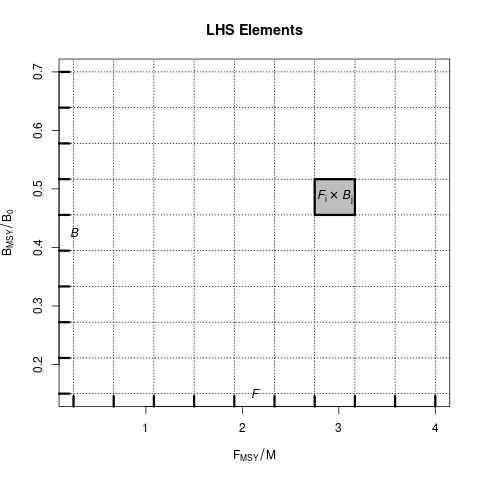
\includegraphics[width=0.49\textwidth]{../gpBias/designGrid.png}
%\vspace{-0.5cm}
%\caption{ LHS grids. Intersecting $\mathcal{F}$ and $\mathcal{B}$ produces $n^2$
%cells; a particular cell $\mathcal{F}_i\times\mathcal{B}_j$ is shown in grey.
%One point is in each of the marginal $\mathcal{F}_i$ and $\mathcal{B}_j$ grid
%elements.
%}
%\end{wrapfigure}
%
%%
%A LHS of size $n$, in the 2 dimensional space defined
%by RPs, distributes samples so as to spread points across a design region in a
%broadly representative way. A LHS design extends the notion of a univariate
%random uniform sample across multiple dimensions so that each margin of the design 
%space enjoys a uniform distribution.
%
%%
%LHS designs achieve this notion of uniformity by first partitioning each dimension 
%of the design space into regular grids of size $n$. By intersecting the grids
%of each dimension, cells are produced that evenly partition the design space.
%In two dimensions $n^2$ cells are produced, from which a total of $n$ samples
%are taken. Crucially only one point is randomly sampled from a given element of
%each grid in each dimension so as to reduce clumping of the $n$ samples across
%the design space.

%
\subsection{Design \label{sLHS}}

%
\begin{wrapfigure}{r}{0.5\textwidth}
%\vspace*{-1.5cm}
%\begin{figure}[h!]
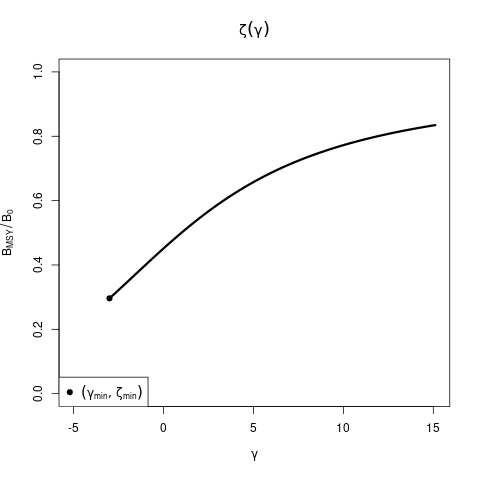
\includegraphics[width=0.5\textwidth]{../gpBias/zeta.png}
\vspace*{-1.3cm}
\caption{$\zeta(\gamma)$ Plotted for $F^*=0.1$ and $M=0.2$. The point
$(\gamma_{min}, \zeta_{min})$ shows the lowest biologically meaningful
value of $\gamma$.} %; below which productivity is negative.}
%\end{figure}
\end{wrapfigure}


%%
%\begin{wrapfigure}{r}{0.5\textwidth}
%%\vspace{-0.5cm}
%\begin{itemize}
%        \item[] \hspace*{-1cm}Given $B_0$, $M$, and $F^*$:
%        \item[1)] Draw $\gamma' \sim \gamma|F^*, M$.
%        \item[2)] Compute $\frac{B^*}{B_0} = \zeta(\gamma')$
%        \item[3)] Compute $\alpha' = \alpha(\gamma', F^*, M)$
%        \item[4)] Compute $\beta' = \beta(\alpha', \gamma', M, B_0)$
%\end{itemize}
%%\vspace{-0.5cm}
%\caption{ An outline of the sampling procedure for $\gamma$
%%(and associated quantities) 
%given $B_0$, $M$, and $F^*$.
%}
%\end{wrapfigure}

%RPs $\mapsto$ $\theta$ or $\theta$ $\mapsto$RPs
Due to the lack of an analytical relationship mapping RPs $\mapsto$ $\theta$,
analogous to the PT model's Eq. (\ref{gammaOfB}), producing a LHD over Schnute 
RPs requires a more tactful approach.
The structured relationship between the RPs and productivity parameters,
described in Section (\ref{sSim}), allows an approximate LHD to be obtained by
a careful navigation of the system of equations seen in Eq. (\ref{abgSys}).

%\clearpage
%
Under the Schnute model, let $\mathcal{F}$ and $\mathcal{B}$ represent regular grids on
%Letting $\mathcal{F}$ and $\mathcal{B}$ be equally spaced grids, of size $n$, on 
\mbox{$\frac{F^*}{M}\in(0.25, 4)$} and \mbox{$\frac{B^*}{B_0}\in(0.15, 0.7)$}
respectively which can serve as the scaffolding for computing an approximate LHS.
Furthermore, let the full design space be defined on the rectangle $R_{full}=(0.25, 4)\times(0.15, 0.7)$.

%
Since it is not practical to invert $\zeta(\gamma)$, a uniform sample in
$\frac{B^*}{B_0}$ can be obtained by modeling $\gamma$ as a random
variable, with realization $\gamma'$, and thinking of $\zeta(\gamma)$ as its
cumulative distribution function (CDF). The aim is to model $\gamma$ as an
easily sampled random variable with a CDF that closely approximates $\zeta$, so
that $\zeta(\gamma')\dot\sim U(\zeta_{min},1)$ as closely as possible. The 
point $(\gamma_{min}, \zeta_{min})$ is the lowest biologically meaningful
value of $\gamma$ and $\frac{B^*}{B_0}$ respectively for a given 
$\frac{F^*}{M}$, below which productivity is negative \cite{myers_maximum_1999, punt_extending_2019}. % defined by the relationship between Schnute productivity and linear natural mortality.
There may be many good models for the distribution of $\gamma$, but in this setting
the following distribution is very effective,
%
%
%\clearpage
%
%
%is very effective,
\begin{align}
\gamma' \sim \zeta_{min}\delta(\gamma_{min}) + t(\mu, \sigma, \nu)\bm{1}_{\gamma>\gamma_{min}}. \label{mixT}
\end{align}

%
Above, $t$ is the density of the three-parameter location-scale family Student's $t$
distribution with location $\mu$, scale $\sigma$, and degrees of freedom $\nu$.
$\bm{1}_{\gamma>\gamma_{min}}$ is an indicator function that serves to truncate the
Student's $t$ distribution at the lower bound $\gamma_{min}$.
$\delta(\gamma_{min})$ is the Dirac delta function evaluated at $\gamma_{min}$,
which is scaled by the known value $\zeta_{min}$; this places probability mass
$\zeta_{min}$ at the point $\gamma_{min}$. Since sampling from a Student's $t$
distribution is readily doable, sampling from a truncated Student's $t$ mixture
only requires slight modification.

%$~$\\$~$\\
Let $T$ be the CDF of the modeled distribution of $\gamma$. Since the point
$(\gamma_{min}, \zeta_{min})$ is known from the dynamics of the Schnute model
at a given RP, full specification of Eq. (\ref{mixT}) only requires determining
the values for $\mu$, $\sigma$, and $\nu$ which make $T$ best approximate
$\zeta(\gamma)$. Thus, the values of $\mu$, $\sigma$, and $\nu$ are chosen by
minimizing the $L^2$ distance between $T(\gamma)$ and $\zeta(\gamma)$.
%Letting $T$ be the CDF of the modeled distribution of $\gamma$, the values of $\mu$, $\sigma$, and $\nu$ are chosen by minimizing the $L^2$ distance between $T(\gamma)$ and $\zeta(\gamma)$.
%{\gamma_{min}}^{\gamma_{0.9}}

%\vspace{-0.125cm}
\begin{align}
[\hat\mu, \hat\sigma, \hat\nu]=\underset{{[\mu, \sigma, \nu]}}{\arg\min}\int_\Gamma \big(T(\gamma; \mu, \sigma, \nu) - \zeta(\gamma)\big)^2 d\gamma
\end{align}

%{\color{red}
%\cite{punt_extending_2019} \cite{myers_maximum_1999} define $(\gamma_{min}, \zeta_{min})$
%}

%\clearpage
\vspace{-0.25cm}
%
\begin{wrapfigure}{R}{0.5\textwidth}
	\renewcommand{\baselinestretch}{1.3}
        %\vspace{-0.5cm}
        \vspace{-1cm}
        \begin{minipage}{0.5\textwidth}
                \begin{algorithm}[H]
                        \caption{LHS of size $n$ on rectangle $R$.}
                        \label{lhsAlg}
                        \begin{algorithmic}[1]
                        \Procedure{$LHS_n(R)$}{}
                        \State Define $n$-grids $\mathcal{F}, \mathcal{B}\in R$
                        \For{each grid element $i$}
                        \State Draw $\frac{F^*}{M} \sim Unif(\mathcal{F}_i)$
                        \State Compute $[\hat\mu, \hat\sigma, \hat\nu]$ given $F^*~\&~M$
                        \While {$\mathcal{B}_j$ not sampled}
                                \State Draw $\gamma' \sim T(\gamma|\hat\mu, \hat\sigma, \hat\nu)$
                                \State Compute $\zeta' = \zeta(\gamma')$
                                \State Compute $j$ such that $\zeta'\in\mathcal{B}_j$
                                %\State Compute $\alpha^* = \alpha(\gamma^*, F^*, M)$ 
                                %\State Compute $\beta^* = \beta(\alpha^*, \gamma^*, M, B_0)$   
                                %\State \mbox{Save $(\frac{F^*}{M}, \zeta^*)\Leftrightarrow(\alpha^*, \beta^*, \gamma^*)$ in $\mathcal{F}_i\times\mathcal{B}_j$} 
                        \EndWhile
                        \State Compute $\alpha' = \alpha(\gamma', F^*, M)$
                        \State Compute $\beta' = \beta(\alpha', \gamma', M, B_0)$
                        \State \mbox{Save $(\frac{F^*}{M}, \zeta')\Leftrightarrow(\alpha', \beta', \gamma')$ in $\mathcal{F}_i\times\mathcal{B}_j$}
                        \EndFor
                        \EndProcedure
                        \end{algorithmic}
                \end{algorithm}
        \end{minipage}
\end{wrapfigure}
\renewcommand{\baselinestretch}{2.5}
%{\color{red}Connect $T(\gamma|\hat\mu, \hat\sigma, \hat\nu)$ to overall algorithm.}

%Furthermore, $T(\gamma|\hat\mu, \hat\sigma, \hat\nu)$, taken together with 
The distribution $T(\gamma|\hat\mu, \hat\sigma, \hat\nu)$ is fit for use in
generating $\gamma'$ random variates at a specific $F^*$ and $M$. This
approximation releases the need to invert $\zeta$ w.r.t. $\gamma$ by using
the $\gamma'$ samples to generate approximatly uniform samples of
$\zeta(\gamma')$. By sampling approximatly uniform $\zeta(\gamma')$ random
variates in this way, and making use of the structure in Eq. (\ref{abgSys}), %allows for the collection of 
an approximate LHS can be collected via \mbox{Algorithm (\ref{lhsAlg}).} %Figure (\ref{sudoCode}). 

%
For a given $i$, $\frac{F^*}{M}$ is drawn uniformly from within $\mathcal{F}_i$. Conditioning on the
sample of $F^*$, and $M$, $T(\gamma|\hat\mu, \hat\sigma, \hat\nu)$ is fit and
$\gamma'$ is sampled. $\zeta'$ is then computed and placed into the appropriate
grid element $\mathcal{B}_j$. Given $\gamma'$, the cascade $\alpha(\gamma')$,
and $\beta(\alpha(\gamma'), \gamma')$, can be computed. The algorithm
continues until all of the design elements, \mbox{$(\frac{F^*}{M}, \zeta')\Leftrightarrow(\alpha', \beta', \gamma')$,}
have been computed for all $i\in[1,...,n]$.

%
%\clearpage
\subsubsection{Design Refinement\label{desRef}}

%
Since the behavior of RP inference, under misspecified models, will vary in
yet-unknown ways, the exact sampling design density may be hard to know a priori.
Several factors, including the particular level of observation uncertainty,
high variance (i.e. hard to resolve) features of the response surface, or
simply "gappy" instantiations of the initial LHD may necessitate
adaptive design refinement, to accurately describe RP biases. Given the
temperamental relationship between RPs and productivity parameters in the
Schnute model, a recursive refinement algorithm that makes use of the
previously described LHS routine, is developed.

%
While LHS ensures uniformity in the design margins, and a certain degree of spread,
it is widely recognized that particular LHD instantiations may leave substantive gaps
in the simulation design. To correct this, LHD are often paired with design elements
of maximin design \cite{morris_exploratory_1995,devon_lin_latin_2015}. Maximin designs sample
the design space by maximizing the minimum distance between sampled points.
This has the advantage of definitionally filling holes in the design, %\shortcite{johnson_minimax_1990}, %in a way that has been %shown to have asymtoptically optimal characteristics for Gaussian process models \shortcite{johnson_minimax_1990}
however because no points are ever drawn outside of the design domain, samples tend to
clump around edges (particularly corners) of the design domain. Since LHS ensures
uniformity in the margins and maximin designs enjoys a certain sense of optimality 
in how they define and fill gaps \cite{johnson_minimax_1990}, the methods are 
quite complimentary when combined.

%Thus 
Making use of this complimentary relationship, holes in the existing RP LHD %LHS design of RPs 
are identified based on maximin design principles.
%Holes in the existing design are identified based on maximin design principles.
%That is to say,
New design points are collected based on areas of the RP design
space which optimize the maximin dinstance %maximizes the minimum distance 
between all pairs of points in the
{current design, based on the following distance function}
%$\mathcal{F}$ and $\mathcal{B}$
\begin{align}
d(\bm{x}, \bm{x'}) &= \sqrt{(\bm{x}-\bm{x'})^T\bm{D}^{-1}(\bm{x}-\bm{x'})}\\
\bm{D} &= \bm{\mbox{diag}\left[} \big(max(\mathcal{F})-min(\mathcal{F})\big)^2, ~\big(max(\mathcal{B})-min(\mathcal{B})\big)^2 \bm{\right]}. \nonumber
\end{align}

%
Above, $d$ is a scaled distance function that defines the distance between
points in the differing scales of $\frac{B^*}{B_0}$ and $\frac{F^*}{M}$.
$\bm{D}$ is a diagonal matrix that measures the squared size of the domain in each 
axis of so as to normalize distances to a common scale.
%the domain for use normalizing distances to a common scale.
%Since the scales of $\frac{B^*}{B_0}$ and $\frac{F^*}{M}$ differ, the 
%distance function 

%
If $\bm{X_n}$ is the initial design, computed on $R_{full}$, let $\bm{x_a}$ be the 
augmenting point which maximizes the minimum distance between all of the existing
design points,
%
\begin{align}
        %x_a = \argmax_{x'} ~\min\{ ||x_i-x'||^2: i=1,...,n \}
        \bm{x_a} = \argmax_{\bm{x'}} ~\min\{ d(\bm{x_i}, \bm{x'}): i=1,...,n \}.
\end{align}
%

%
The point $\bm{x_a}$ is used as an anchor for augmenting $\bm{X_n}$. %by collecting 
An additional $LHS_{n'}$ (via Algorithm (\ref{lhsAlg})) is collected, adding
$n'$ design points, centered around $\bm{x_a}$, to the overall design. %are collected, %$LHS_{n'}$ is collected, using Algorithm (\ref{lhsAlg}). 
The augmenting region %(for collecting $LHS_{n'}$)
, $R_{(x_a, d_a)}$, is defined
based on the square centered at $\bm{x_a}$ with side length $2d_a$, where
\mbox{$d_a = \min\{ d(\bm{x_i}, \bm{x_a}): i=1,...,n \}$}, in the space defined
by the metric $d$.
%that circumscribes the circle (in the space, defined by the metric $d$) 
%at point $\bm{x_a}$ with radius \mbox{$d_a = \min\{ d(\bm{x_i}, \bm{x_a}): i=1,...,n \}$}.
%
%A $LHS_{n'}$ is collected, using Algorithm (\ref{lhsAlg}), on the rectangle in 
%RP-space that circumscribes the circle (in the space, defined by the metric $d$) 
%at point $\bm{x_a}$ with radius \mbox{$d_a = \min\{ d(\bm{x_i}, \bm{x_a}): i=1,...,n \}$}.
%%in the space defined by the metric $d$.

%
Due to the tendency of maximin sampling to cluster augmenting points on the edges
of the design space, $R_{(x_a, d_a)}$ is truncated by the outer most limits of
$R_{full}$ so as to focus design augmentation within the specified domain of the
simulation. Furthermore, since the design space has a nonlinear constraint at low
values of $\frac{B^*}{B_0}$, the calculation of $x_a$ is further truncated
based on a convex hull defined by the existing samples in the overall design.

%
Design refinement then proceeds as follows. An initial design is computed on the 
full RP design space, $X_{n} = LHS_{n}(R_{full})$. % design is computed 
%based on an overall simulated region of RPs $R_{full}$. 
The maximin augmenting point, $x_a$, is computed at a maximin distance of $d_a$ 
from the existing samples. An augmenting design $X_{n'} = LHS_{n'}(R_{(x_a, d_a)})$ 
is collected and added to $X_n$. Design refinement carries on recursively 
collecting augmenting designs in this way until the maximin distance falls 
below the desired level.

{\color{red} State how small in practice here.}

%
\subsection{\color{red}refer back to GP?}

%
\section{Results}

%
\subsection{Design}

%
\begin{wrapfigure}{r}{0.45\textwidth}
%\vspace{-3cm}
\vspace{-2cm}
%\begin{figure}[h!]
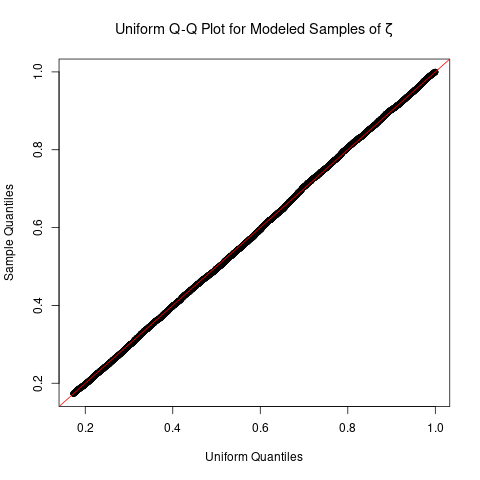
\includegraphics[width=0.45\textwidth]{../gpBias/qqUnif.png}
\vspace{-1cm} %against theoretical uniform quantiles
\caption{Uniform Q-Q plot for $\zeta$ plotted for $F^*=0.1$ and $M=0.2$.}
\label{qqZeta}
%\end{figure}
\end{wrapfigure}

%
Algorithm (1) enforces uniform marginals in $\frac{F^*}{M}$ directly, as well
as the adherence of the overall design to latin squares.
Figure (\ref{qqZeta}) shows a uniform Q-Q plot for sampled $\zeta$, using
Algorithm (1), against theoretical uniform quantiles. As evidence by the
excellent coherence to the theoretical uniform quantiles, the approximation
in Section (\ref{sLHS}) for sampling $\gamma$ (and therefore $\zeta(\gamma$)),
%for the purpose of computing $\zeta(\gamma$), 
is very effective.
Furthermore since numerical inversion of $\zeta(\gamma)$ is costly and
unreliable, the relative speed and accuracy that this approximate LHS sampling
method provides is pivotal for the rest of the work presented here. %to understanding the relationship between RPs and $\gamma$.

%
\begin{wrapfigure}{r}{0.5\textwidth}
\vspace{-0.5cm}
%\begin{figure}[h!]
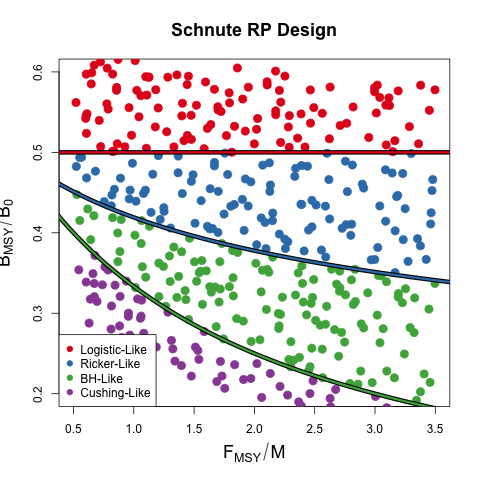
\includegraphics[width=0.5\textwidth]{../ddBias/designLineColorHHardFlatT30N150WWideN112.png}
%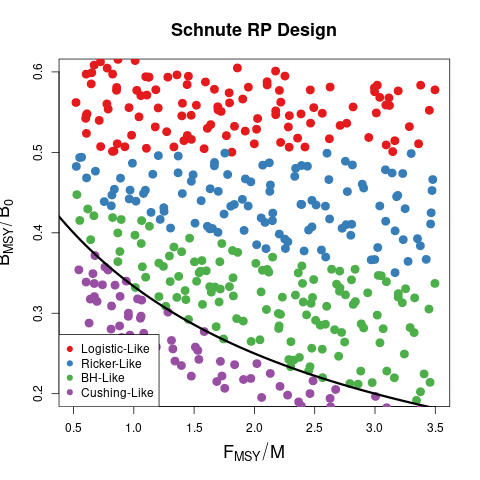
\includegraphics[width=0.5\textwidth]{../gpBias/designLineColorHHardFlatT30N150WWideN112.png}
%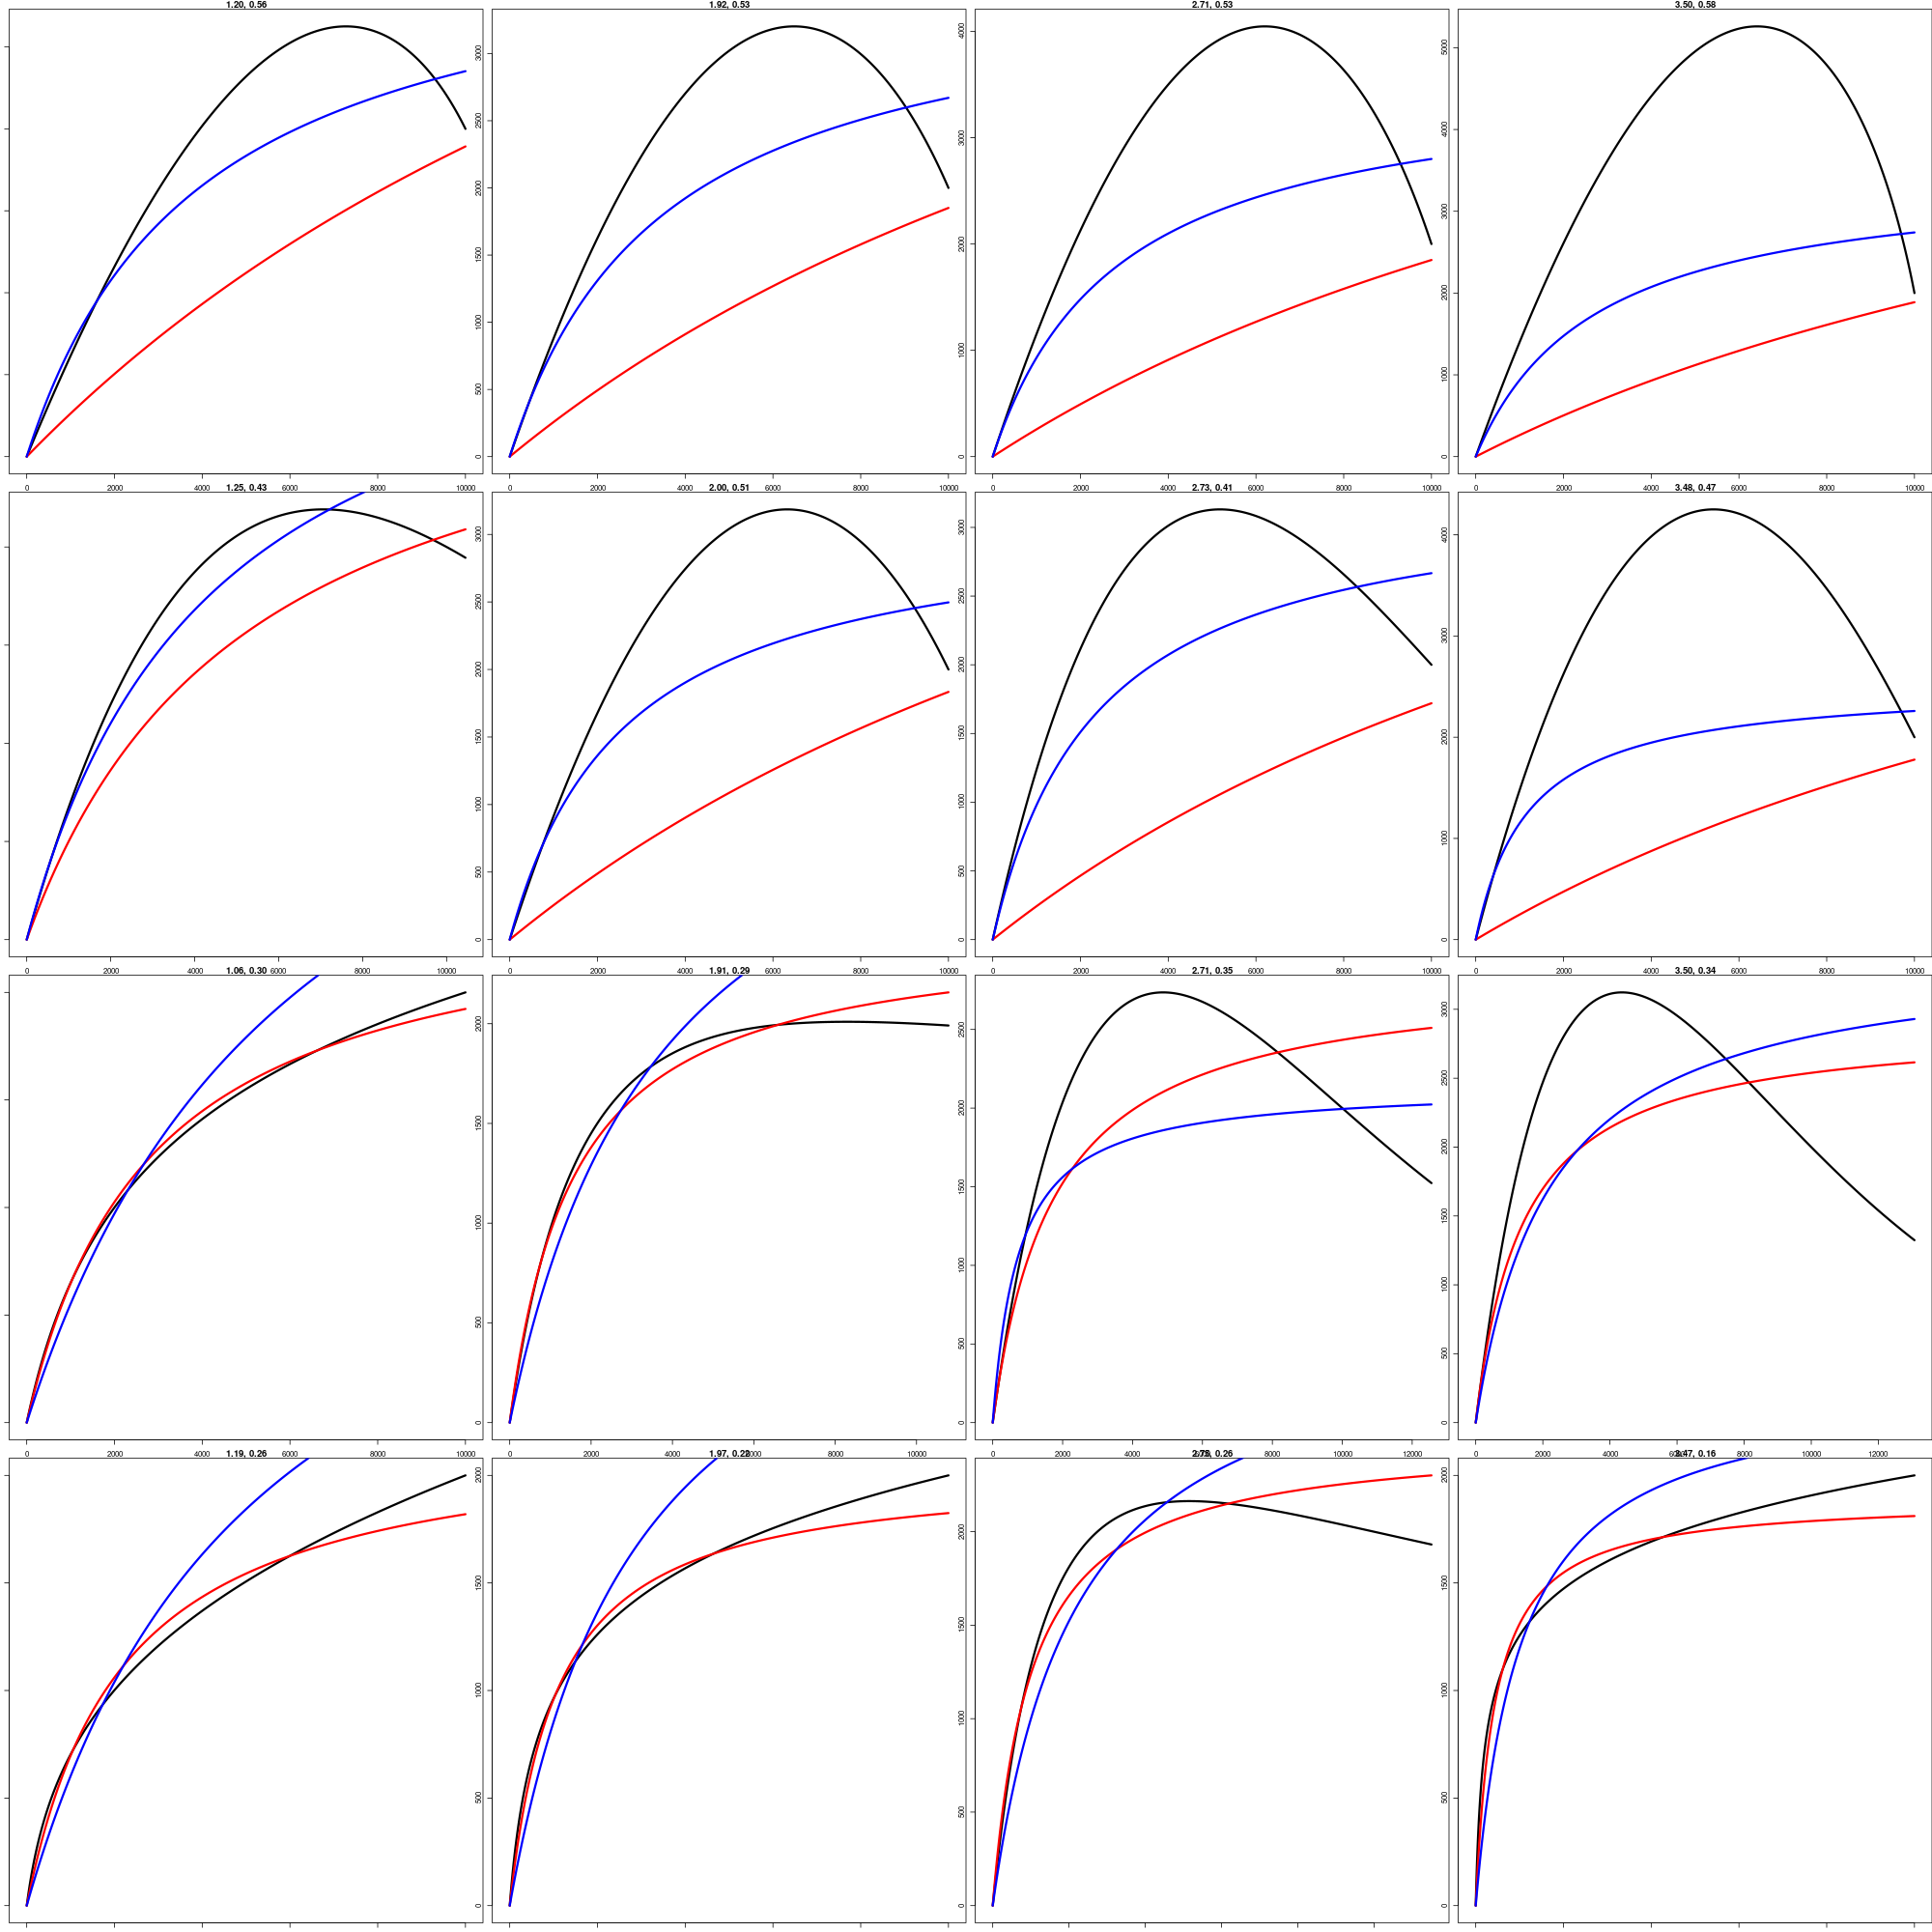
\includegraphics[width=0.5\textwidth]{../gpBias/rGridHHardFlatT30N150WWideN112.png}
\vspace{-1cm}
\caption{
A Schnute RP design. % resulting from design refinement of Algorithm (1). 
Colors indicate different regimes of Schnute production. % function.
%Samples are colored by the ranges the $\gamma$ parameter which result in 
%different regimes of the Schnute production function.
The black curve shows the BH set.
}
\label{colorDes}
%\end{figure}
\end{wrapfigure}

%
Similarly to the PT model, the three-parameter Schnute model is uniquely
identified by each point in the space of $\frac{F^*}{M}$
and $\frac{B^*}{B_0}$ RPs. As seen in Figure (\ref{colorDes}), Schnute
production has different behaviors in different ranges of RPs space, which
are entirely defined by the value of $\gamma$ (shown in Figure (\ref{sRegimes})).
%As shown in Figure (\ref{sRegimes}), as well as the colors of Figure (\ref{colorDes}), 
When $\gamma\ge1$ the Schnute model produces a family of Logistic-like curves that are
increasingly right leaning as $\gamma$ increases.
For $1>\gamma\ge0$, Schnute production takes a family of left leaning Ricker-like curves
that all, at least, approach the x-axis. For $0>\gamma>-1$ there are a family of BH-like
curves that do not approach the x-axis but still have decreasing productivity for large
biomass stocks. When $\gamma$ is exactly $-1$ Schnute reduces to BH production which has
asymptoting production for large biomass. Finally when $-1>\gamma$ Schnute
produces a family of increasing Cushing-like curves that do not asymptote, and produces
linear production as $\gamma\to-\infty$.

%
Modeling index data that are simulated broadly over the theoretical space of RPs
with misspecified BH production greatly limits the range of possible RPs that
can be inferred. Under BH production the full theoretical space of RPs are
limited to the curve \mbox{$\frac{B^*}{B_0}=\frac{1}{F^*/M+2}$.} Define the
``BH set'' as the set of RPs defined by this limited space, i.e. the curve \\
$\left\{\left(\frac{F^*}{M}, \frac{B^*}{B_0}\right) \;\middle|\; \frac{B^*}{B_0}=\frac{1}{F^*/M+2}\right\}$.
as seen in the {\color{red}black curve} in Figure (\ref{colorDes}).
The farther away from this set that Schnute data are simulated, the more the
BH model is misspecified for those data.

%
\subsection{Metamodeled Trends}

{\color{red} \cite{punt_extending_2019} \cite{myers_maximum_1999} for the bottom left corner

The Deriso–Schnute model (Hilborn and Walters 1992),
an alternative three-parameter model, has the Ricker and the
Beverton–Holt as special cases. However, it suffers from the
same problems that we described above: survival is not constrained to be finite 
except when the model is a Ricker model, or it has the derivative of survival 
as S → 0 constrained to be zero.

Punt \& Cope
The cells in red indicate combinations of FMSY/M and BMSY/B0 for which 
recruitment is negative for 0<B<B0
}

%
Unlike the Schaefer model, the BH set is not a constant in
$\frac{B^*}{B_0}$. Under the BH model, bias in $\frac{B^*}{B_0}$ is no
longer entirely defined by the degree of model misspecification, but rather the
structure of BH RPs allows bias in both $\frac{B^*}{B_0}$ and $\frac{F^*}{M}$
to interact as a function of contrast in the data.
%This has the effect of allowing the bias in $\frac{B^*}{B_0}$ and $F^*$ 

%
\begin{figure}[h!]
\begin{minipage}[h!]{0.49\textwidth}
\hspace*{-0.5cm}
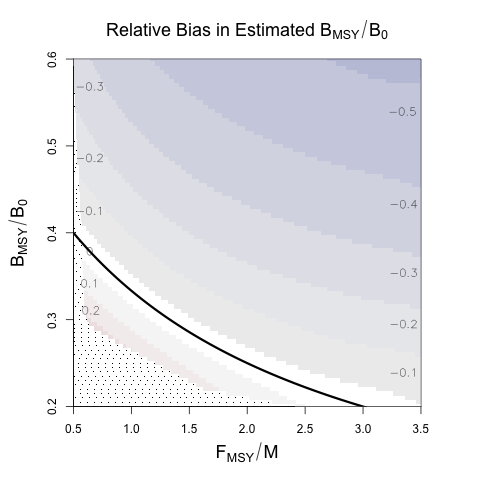
\includegraphics[width=1.1\textwidth]{../gpBias/zetaRelBiasSchnuteExpT45N150Wide.png}\\
%\hspace*{1cm}
\caption{\label{contrastTrio}
Heatplots showing the bias in RP estimation induced by model misspecification of
the BH model in the high contrast simulation setting.
In all cases the restricted RP-space of the BH set is shown as the black curve.
(\emph{left}) Relative bias in $\frac{B^*}{\bar B(0)}$.  (\emph{top-right})
Bias in RP-space shown directionally. Arrows point from the location where
data is generated, toward the location in the BH set where MLE projects estimated
RPs. The intensity of color represents the excess bias relative
to the shortest possible mapping. (\emph{bottom}) Relative bias in $F^*$.
}
$~$\\$~$\\
\end{minipage}
\begin{minipage}[h!]{0.49\textwidth}
\hspace*{1cm}
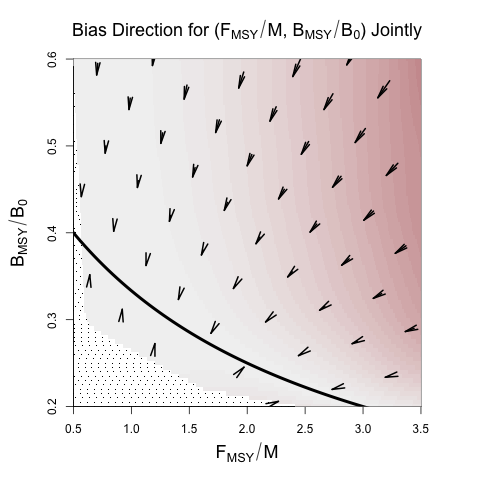
\includegraphics[width=1.1\textwidth]{../gpBias/directionalBiasSchnuteSubTitleExpT45N150Wide.png}\\
\hspace*{1cm}
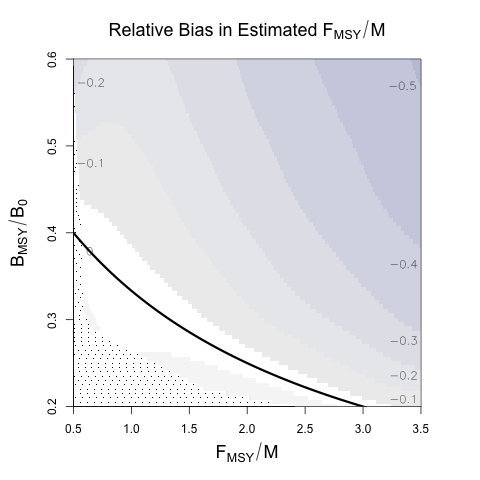
\includegraphics[width=1.1\textwidth]{../gpBias/fMSYRelBiasSchnuteExpT45N150Wide.png}
\end{minipage}
\end{figure}

%\paragraph{High Contrast}
\subsubsection{High Contrast}

%
Figure (\ref{contrastTrio}) shows metamodeled RP bias surfaces for inference
under the BH model in the high contrast setting. The (\emph{left}) and
(\emph{bottom}) panels focus only on the $\frac{B^*}{\bar B(0)}$ and
$\frac{F^*}{M}$ components of bias respectively. In these panels bias is shown
as relative bias, $\frac{\widehat{RP}-RP}{RP}$, similar to a percent error calculation.
Where $RP$ represents the true value of the three-parameter RP, and $\widehat{RP}$ 
refers to the metamodel estimate.

%
Figure (\ref{contrastTrio}, \emph{top-right}) combines the components of bias to
show the overall mapping of RPs under BH inference in the high contrast
simulation setting. Unlike high contrast RP inference under the Schaefer model,
where maily bias in $\frac{B^*}{\bar B(0)}$ occured, the BH model does shows
bias in both RPs here. Despite the bias in $\frac{B^*}{\bar B(0)}$ and
$\frac{F^*}{M}$ these results are similar to that of the Schaefer model in
that the overall mapping of RPs is very nearly a minimal distance mapping onto
the constrained set of RPs. %In this setting the 
The primary difference between Schaefer model and BH RP inference is the
geometry of their limited RP spaces. Unlike the Schaefer model the BH set
encouragesbias in both RPs for misspecified models even in very well informed
setting.

\subsubsection{Low Contrast}

%
\begin{wrapfigure}{r}{0.5\textwidth}
\vspace{-0.5cm}
%%\vspace{-1.25cm}
%\begin{figure}[h!]
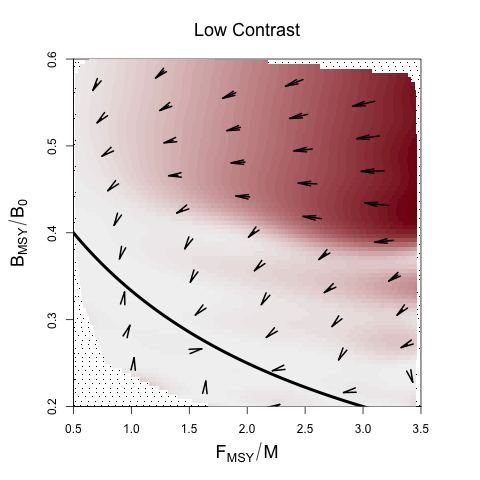
\includegraphics[width=0.5\textwidth]{../gpBias/directionalBiasSchnuteSubHHardFlatT30N150WWideN112.png}
%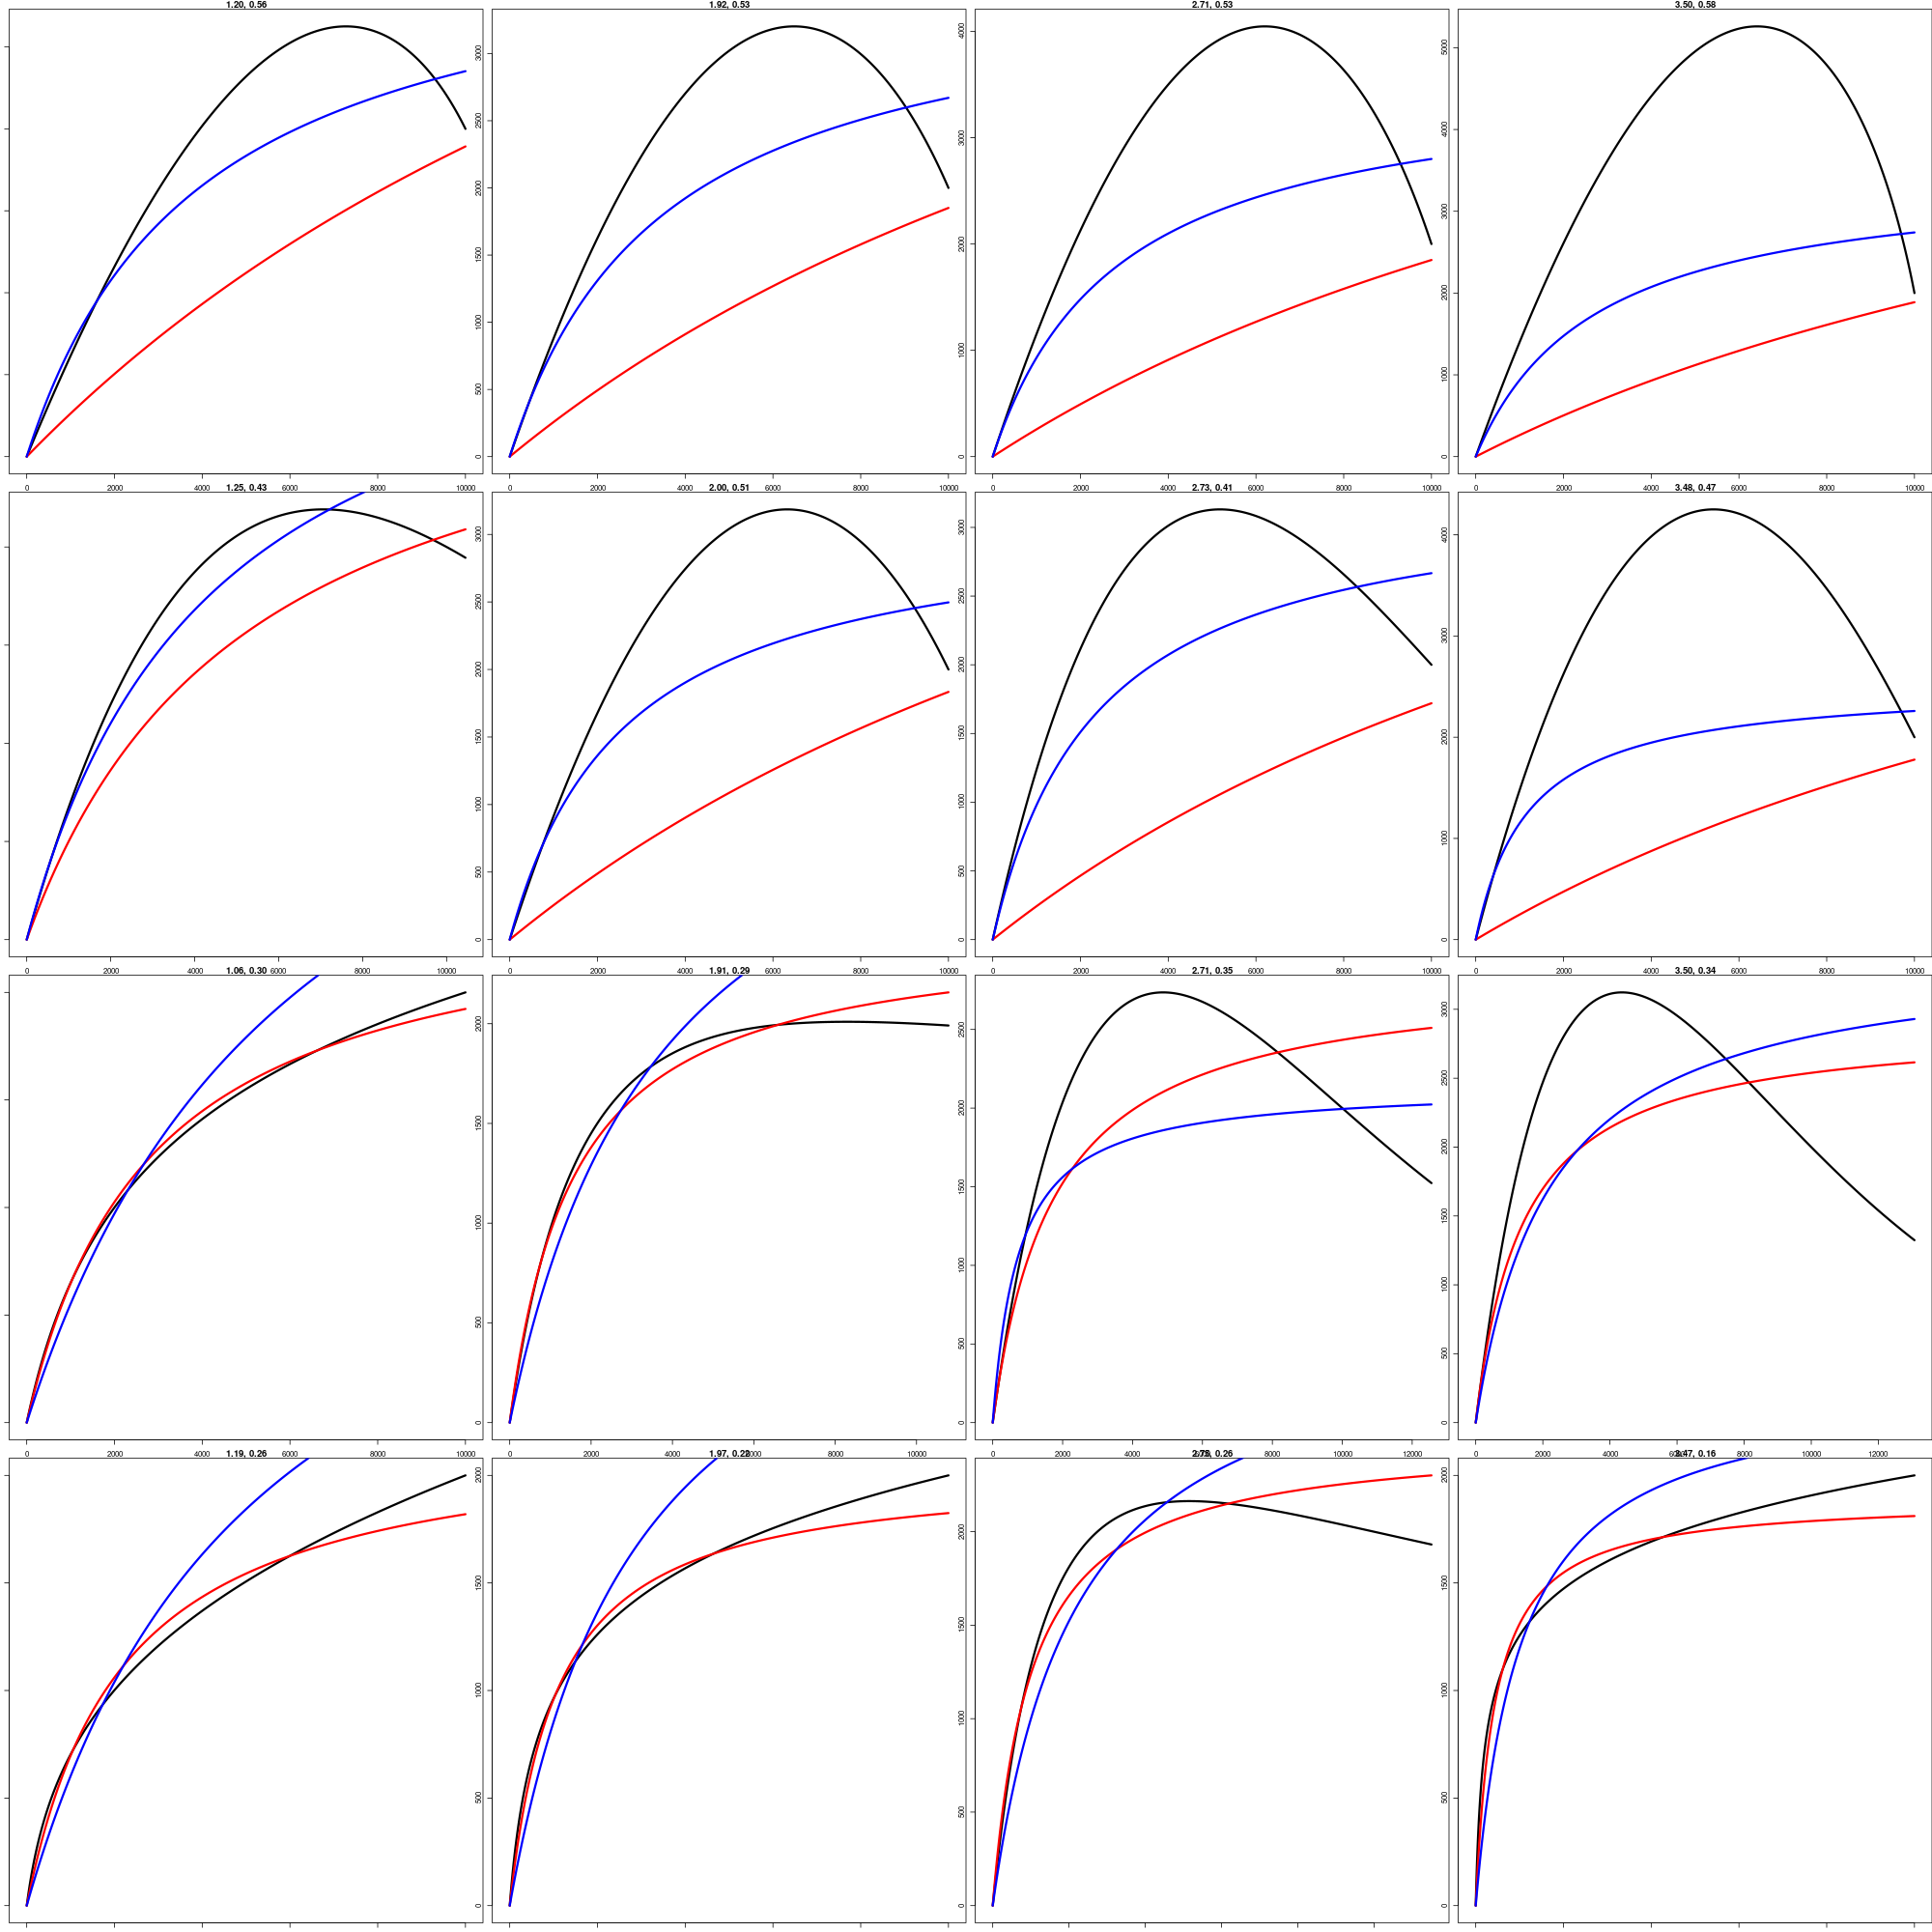
\includegraphics[width=0.5\textwidth]{../gpBias/rGridHHardFlatT30N150WWideN112.png}
\vspace{-1cm}
\caption{
%Relative bias in $F^*$ in the high contrast simulation setting. The BH set is also shown in black. 
Joint bias direction of RP inference in the low contrast simulation setting.
The intensity of color represents the excess bias relative
to the shortest possible mapping.
}
\label{bhLowArrows}
%\end{figure}
\end{wrapfigure}

%
Figure (\ref{bhLowArrows}) shows the mapping of RPs in the low contrast
simulation setting. Figures (\ref{bhLowArrows}) and (\ref{contrastTrio},
\emph{top-right}) share a common scale for the intensity of color to
facilitate comparison. In Figure (\ref{bhLowArrows}) notice that the mildly
misspecified area around the BH set produces mappings onto the BH set which
resemble the minimal distance mapping seen in the high contrast setting. % %in Figure (\ref{contrastTrio}, \emph{top-right}). %
The primary difference in this low contrast setting, is the break point
around $\frac{B^*}{\bar B(0)}=0.4$ above which $\frac{F^*}{M}$ is sharply
underestimated.

%
The region of RPs where the BH model manages to recover the minimal distance
mapping may be considered a ``safe regime'' of data types that are
reasonably well modeled by a BH model. By comparison of Figure (\ref{bhLowArrows}),
with Figure (\ref{colorDes}), this safe regime of the BH model occurs for data
generated for Cushing-like or BH-like production. While bias of the RPs can still become concerningly large, % here, %(as large as $X$ in the worst case) within this region, 
this region can be considered safe in the sense that even for low contrast data
RP estimation under the the BH model recovers the minimal distance mapping.

%
\begin{wrapfigure}{r}{0.5\textwidth}
\vspace{-0.75cm}
%\begin{figure}[h!]
%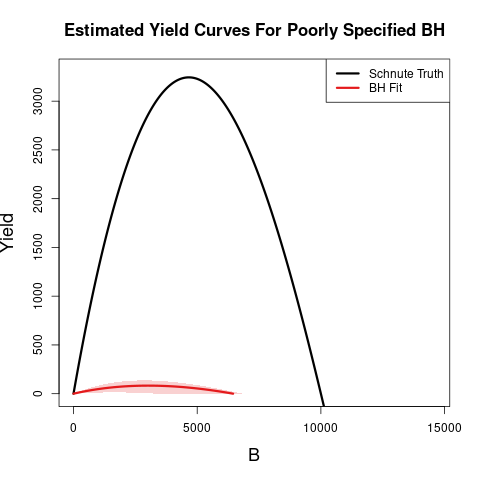
\includegraphics[width=0.5\textwidth]{../gpBias/yeildCurveCompareHHardFlatT30N150WWideN112PrettyX3.4791Z0.4662.png}
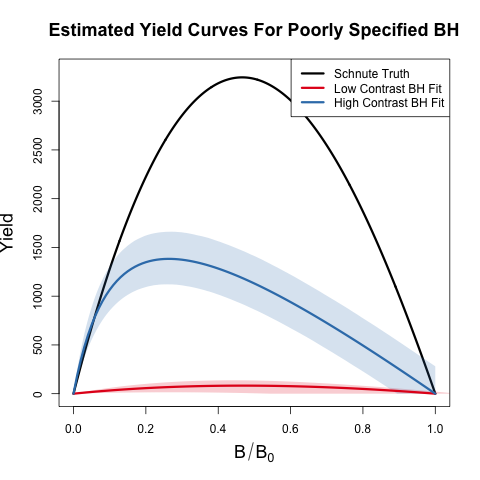
\includegraphics[width=0.5\textwidth]{../gpBias/yeildRelCurveCompareHHardFlatT30N150WWideN112PrettyX3.4791Z0.4662.png}
%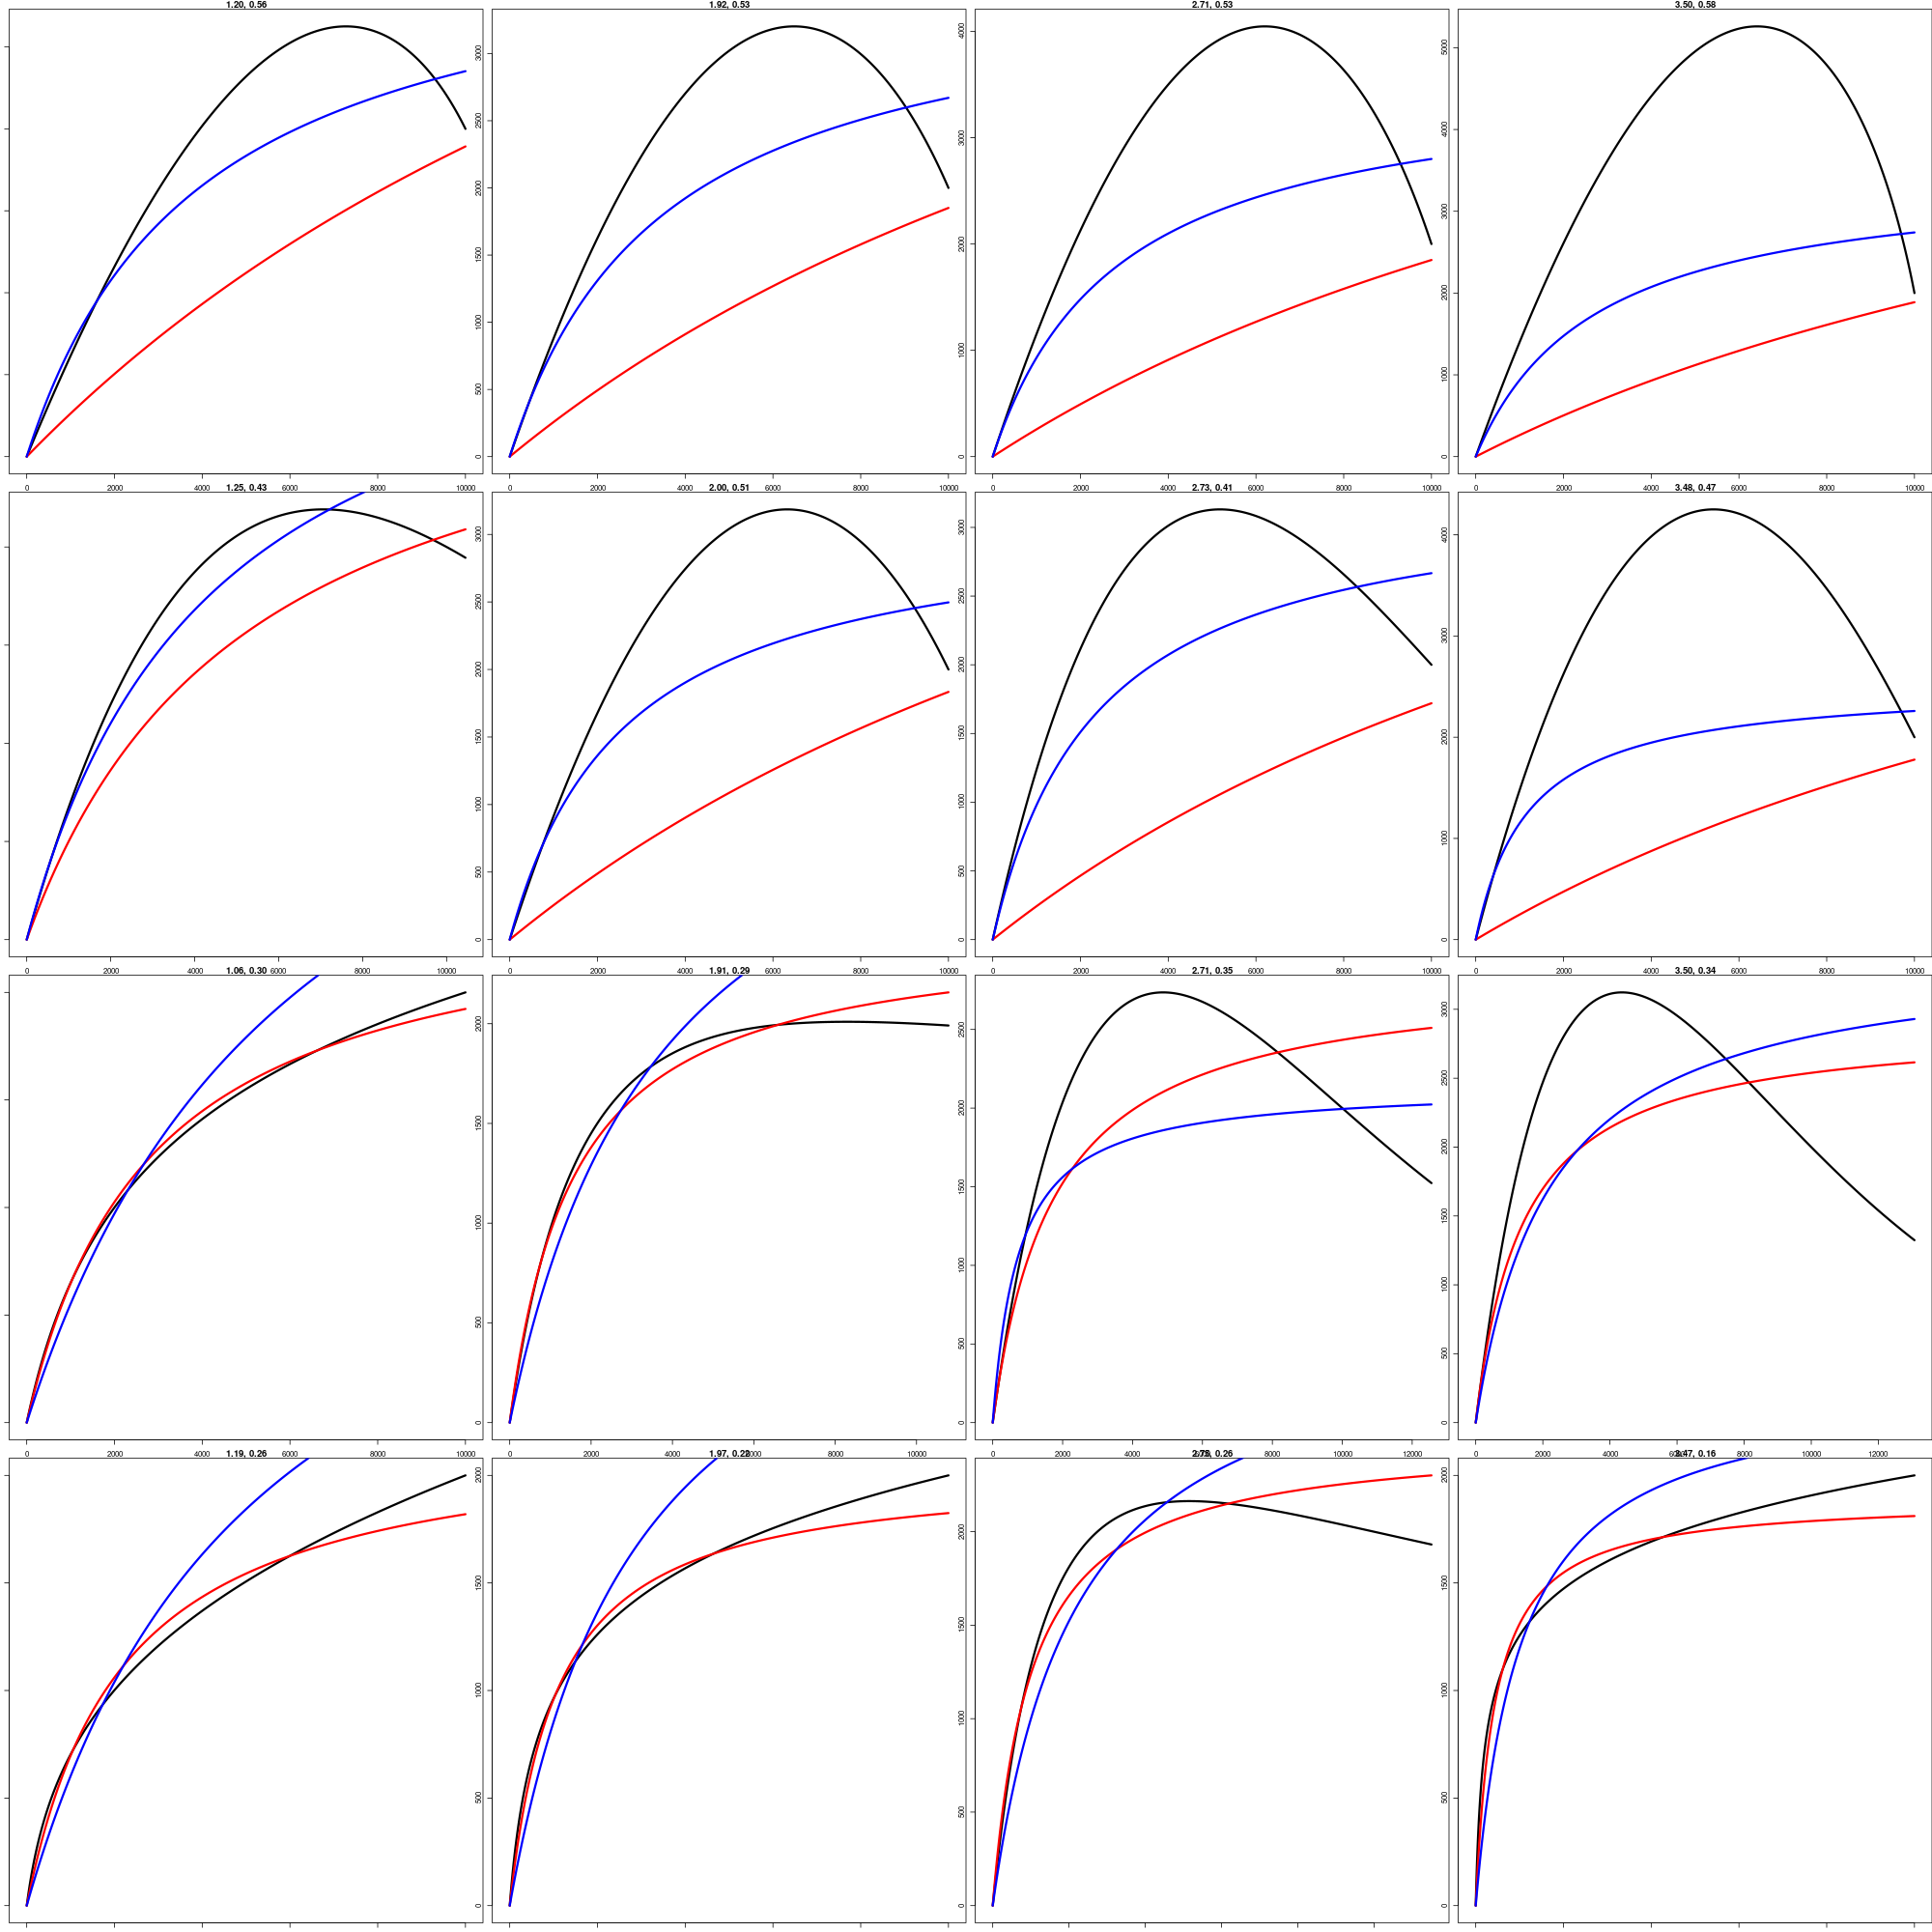
\includegraphics[width=0.5\textwidth]{../gpBias/rGridHHardFlatT30N150WWideN112.png}
\vspace{-1cm}
\caption{
Yield curves for data generated with $\frac{F^*}{M}=3.48$ and $\frac{B^*}{\bar B(0)}=0.48$.
%Convert into $B/B_0$. Show the high contrast curve.
}
\label{bhFmsy}
%\end{figure}
\end{wrapfigure}

%
Outside of this safe regime, RP estimation breaks from the minimal distance mapping
at the interface between BH-Like and Ricker-Like regimes of the Schnute model (again see
Figure (\ref{colorDes})). The Ricker model lies along this regime interface, and
represents the first model to approach the x-axis for large biomasses as $\gamma$
increases. This markedly unBH-like productivity in the low information simulation
setting breaks MLE inference from the minimal distance mapping and instead maps
RPs to extremely low values of $F^*$; consequently $\frac{B^*}{\bar B(0)}$
is estimated near the limiting value under the BH (i.e. $\lim_{F^* \to 0}\frac{1}{F^*/M+2}=0.5$).
Similarly the set of Ricker RPs (as well as the Schaeffer set) include this
trivial limiting point in common ($\frac{F^*}{M}=0$, $\frac{B^*}{\bar B(0)}=0.5$). 

%
Interestingly, in the high contrast setting this trivial mapping for highly
misspecified BH models is not present. This suggests that, under a
misspecified BH model, the presence of adequate information in the data to
produce reasonable estimates of $\frac{F^*}{M}$, drives $\frac{B^*}{\bar B(0)}$
below $0.5$ in accordance with $\frac{B^*}{\bar B(0)}=\frac{1}{F^*/M+2}$,
even when the true $\frac{B^*}{\bar B(0)}>0.5$.
%This suggests that in the presence of adequate 
%information in the data to produce reasonable estimates of $\frac{F^*}{M}$ 
%drives $\frac{B^*}{\bar B(0)}$ away from 0.5, even when the true $\frac{B^*}{\bar B(0)}>0.5$. 
This phenomena balances RP estimation within the constrained BH set as
mediated by the information content of the data and the degree of model
misspecification. When the information content in the data is too small to
drive a compromised RP estimate, inference completely disregards accurate
estimation of $F^*$ in order to better estimate $\frac{B^*}{\bar B(0)}$
by exploiting the common limiting behavior of the BH set and that of
Ricker-like and Logistic-like models.
%may fail by completely disregarding one RP so the sake of preserving whatever 
%similarities may exist between the functional forms of the data and misspecified model. 

%
{\color{red}Add MSY plot}


%
\clearpage
\section{Discussion}

%agree with estimating productivity (steepness, r, etc.)

%extends by LHS simulation design over RPs
%due to the complex failure modes in the low contrast 
%environment the adaptive design is neccessary to make 
%sense of low contrast simulation.
%circumvents lack of analytical RP results
%finds structure in $\alpha$ that enables EJ/Nick paper. 

%extends by LHS simulation design over RPs
%establish different models of model failure from trends in 
\begin{itemize}
\item
Results presented here generally agree with what is known about estimating population
productivity parameters \cite{lee_can_2012, conn_when_2010, magnusson_what_2007}.
\item
These studies appreciate the role of contrast for estimating productivity,
however they struggle to make generally extensible conclusions since they focus only
on a handful of stocks that fall short of forming a random sample of the greater
population of possible stock behaviors.
\item
The LHS design methods presented here are
designed specifically to simulate a representative sample of stocks broadly
across the space of possible RPs.
\item
Furthermore, the simulation design, taken together
with the GP metamodel of productivity parmater estimates, allows this study to control
the degree of model misspecification and generalize conclusions about the behavior
of productivity estimation within the production model setting presented.
\end{itemize}



%
\begin{itemize}
\item 

\end{itemize}



%;
%the simulation design and metamodeling methods presented here further generalize these
%results of these existing results.
%Existing

%{\color{blue} {\it Tease Out BH}\\
%
%%
%Results presented here generally agree with what is known about estimating population
%growth rate parameters \cite{lee_can_2012, conn_when_2010, magnusson_what_2007}.
%These studyies appreciate the role of contrast for estimating growth rates,
%however they struggle to make generally extensible conclusions since they focus only
%on a handful of stocks that fall short of forming a random sample of the greater
%population of possible stock behaviors. The LHS design methods presented here are
%designed specifically to simulate a representative sample of stocks broadly
%across the space of possible RPs. Furthermore, the simulation design, taken together
%with the GP metamodel of productivity parmater estimates, allows this study to control
%the degree of model misspecification and generalize conclusions about the behavior
%of productivity estimation within the production model setting presented.
%
%%%
%%Unfortunately, we are unable to generalize the relationship because the twelve 
%%assessment examples are not a random sample from the population of all fish 
%%stocks and sample size is small. A more general conclusion may be obtained by 
%%including more assessments
%%%
%%\begin{itemize}
%%\item \shortcite{lee_can_2012} Generalizability via random sample of fisheries, LHS RP expli
%%\item multiple starting locations and convergence defined as positive definite Hessian.
%%\end{itemize}
%
%%
%In the presence of contrast, $F^*$ estimation can enjoy very low bias even
%for a wide range of poorly specified models; conversely in the absence of contrast
%$F^*$ estimation can suffer very large bias even for slightly misspecified models.
%This pattern is particularly true for low-contrast inference under the Schaefer model where t
%geometry of the restricted RP set isolates estimation failure of $F^*$ from
%$\frac{B^*}{\bar B(0)}$. While contrast has a similar impact on $F^*$ estimation
%under the BH model, the geometry of the BH RP set correlates estimation bias
%of $F^*$ and $\frac{B^*}{\bar B(0)}$. The GP metamodeling approach reveals a
%more general pattern that highly informative data sets (high contrast)
%produces a nearly minimal distance mapping of RPs %that are nearly minimal distance mapping 
%onto the constrained RP set.
%
%%
%In all cases when model misspecification is removed, even with weakly informative
%data, RP estimation is unbiased and well estimated. Thus contrast alone is
%not the only factor leading to inferential failure. Model misspecification is a
%necessary but not sufficient condition for inducing RP estimation bias. The
%particular RP bias present depends on the RP geometry of the fitted model and
%how that geometry is misspecified relative to the data. The RP mapping is then oriented
%to the RP geometry of the fitted model.
%
%%
%%NOTE: BITCH ABOUT NOT BEING ABLE TO PRODUCE A PERFECTLY INFORMATIVE TIME SERIES
%%SPECULATE ABOUT IDEALLY INFORMATION CATCH PATTERNS (DYNAMIC CALIBRATION OF $F^*$)
%While the relative fishing rate parameterized in Section (\ref{catch}) captures a usefully
%broad spectrum of relevant fishing behaviors, it is still limiting in the amount of informati
%that it can induce. Improved methods for quantifying contrast in fisheries data, and/or metho
%discovering more informative fishing behavior, could improve this analysis. In the absence of
%maximally informative dataset simulation methods will not fully describe how
%inference fails, but the methods presented here tell the most complete picture
%yet, with explicit control of the degree model misspecification, contrast, and
%a simulation design that allows for uniform representative data generation
%across biologically meaningful stocks. The results presented here suggest the
%conjecture that under a maximally informative dataset, RP inference with a two
%parameter production function will be biased in the direction a shortest distance
%map from the true RPs onto restricted set of RPs under the two-parameter model.
%
%%
%Given the potential for model misspecification of RPs, a minimal distance
%mapping of RPs represents a best-case scenario where the total bias of RPs,
%when measured jointly, is minimized. That said, without recognizing the
%geometry of how two-parameter models of productivity limit RP space this may
%lead to unintuitive implications in RP estimation. For example, due to the
%shape of the BH RP set a minimal distance mapping ensures that if there is
%bias in one of $\frac{B^*}{B_0}$ or $F^*$, there will necessarily be
%bias in the other RP. However under the Schaefer model, since the RP set is a
%constant in $\frac{B^*}{B_0}$, bias in $F^*$ is not adulterated in the
%same way by bias in $\frac{B^*}{B_0}$ estimation. While models with
%constant RPs, such as the logistic model $\frac{B^*}{B_0}=\frac{1}{2}$ or
%the Fox model $\frac{B^*}{B_0}=\frac{1}{e}$, are extremely limited, they
%can be valuable tools for developing intuition precisely because they isolate
%RP estimation in their free RPs from the correlated RP biases present in
%models like the BH or Ricker model.
%
%%
%When one considers the implications of RP bias, overestimation of RPs carries
%the severe implication of management recommendations potentially leading to
%overfishing, while underestimation of RP leads to overly conservative management.
%In this sense, when the true model is not known, the geometry of the BH set together
%with the metamodeled bias trends makes the BH model a naturally conservative
%estimator of RPs for most stocks. For most non-BH populations the BH model is
%likely to make conservative errors in its estimates of $F^*$ and $\frac{B^*}{B_0}$.
%The one notable exception to the conservatism of the BH model stands for data
%generated in the Cushing-like regime of Schnute RPs. In this regime the BH
%model tends to be fairly unbiased overall, however the bias that is present
%for these populations tends to be overestimation in both RPs, leading to much
%more severe management consequences for those populations.
%
%%
%The RP bias trends of the Schaefer model demonstrate much less {\color{red}conservatism} than
%For any population with $\frac{B^*}{B_0}<0.5$, $\frac{B^*}{B_0}$ will be overestimated.
%When the population comes from the regime where $\frac{B^*}{B_0}>0.5$, $\frac{B^*}{B_0}$
%will be under estimated, but $F^*$ is likely to be overestimated depending on the degree of
%contrast present in the data. So while the Schaefer model is an intuitive model, it tends to
%lead to much less conservative RP estimation.
%
%%
%While it is important to recognize these limitations of two-parameter models
%of productivity, we should not solely accept conservativism as a rational of
%choosing a BH model of productivity. %Ultimately accuracy of RP estimation, 
%%without structural RP biases, %and accurate assessment of uncertainty is a better state 
%Increasing the flexibility of the production function by moving toward
%three-parameter models would release the underlying structural limitations
%\cite{mangel_perspective_2013} that cause these RP biases in the first place.
%Punt \& Cope \cite{punt_extending_2019} %(Mangel et al., 2013). Punt and Cope (2019) 
%considers a suite of possible three-parameter curves which could be used
%instead of current two-parameter curves. For all of their benefits, three
%parameter production functions have their own complicating factors, and the
%structure present in the Schnute model explored here makes it an intuitive bridge
%model for developing three-parameter models going forward.
%
%}


